\chapter{The Large Hadron Collider and the Compact Muon Solenoid}
\label{ch:LHCCMS}

The LHC is primarily a proton-proton circular collider, situated at the Conseil Europ$\acute{\text{e}}$en pour la Recherche Nucl$\acute{\text{e}}$aire (CERN) on the French-Swiss border. 
It is built 100\m{} underground in the tunnels that housed the Large Electron-Positron (LEP) collider and is currently the largest machine in the world, with an accelerator ring 27\km{} in circumference. 
There are four main experiments operating at the LHC; two multipurpose general detectors, CMS and ATLAS; a precision \bquark{} physics experiment (LHCb); and finally a detector dedicated to heavy ion physics, A Large Ion Collider Experiment (ALICE). 
The full accelerator complex at CERN is shown in Fig.~\ref{fig:CERNcomplex}.
This chapter will highlight a brief history of the LHC, how it is operated to produce collisions in the experimental caverns and the current data-taking environment.
A description is given of the subdetectors that form the CMS experiment.
\begin{figure}[htpb]
	\centering
	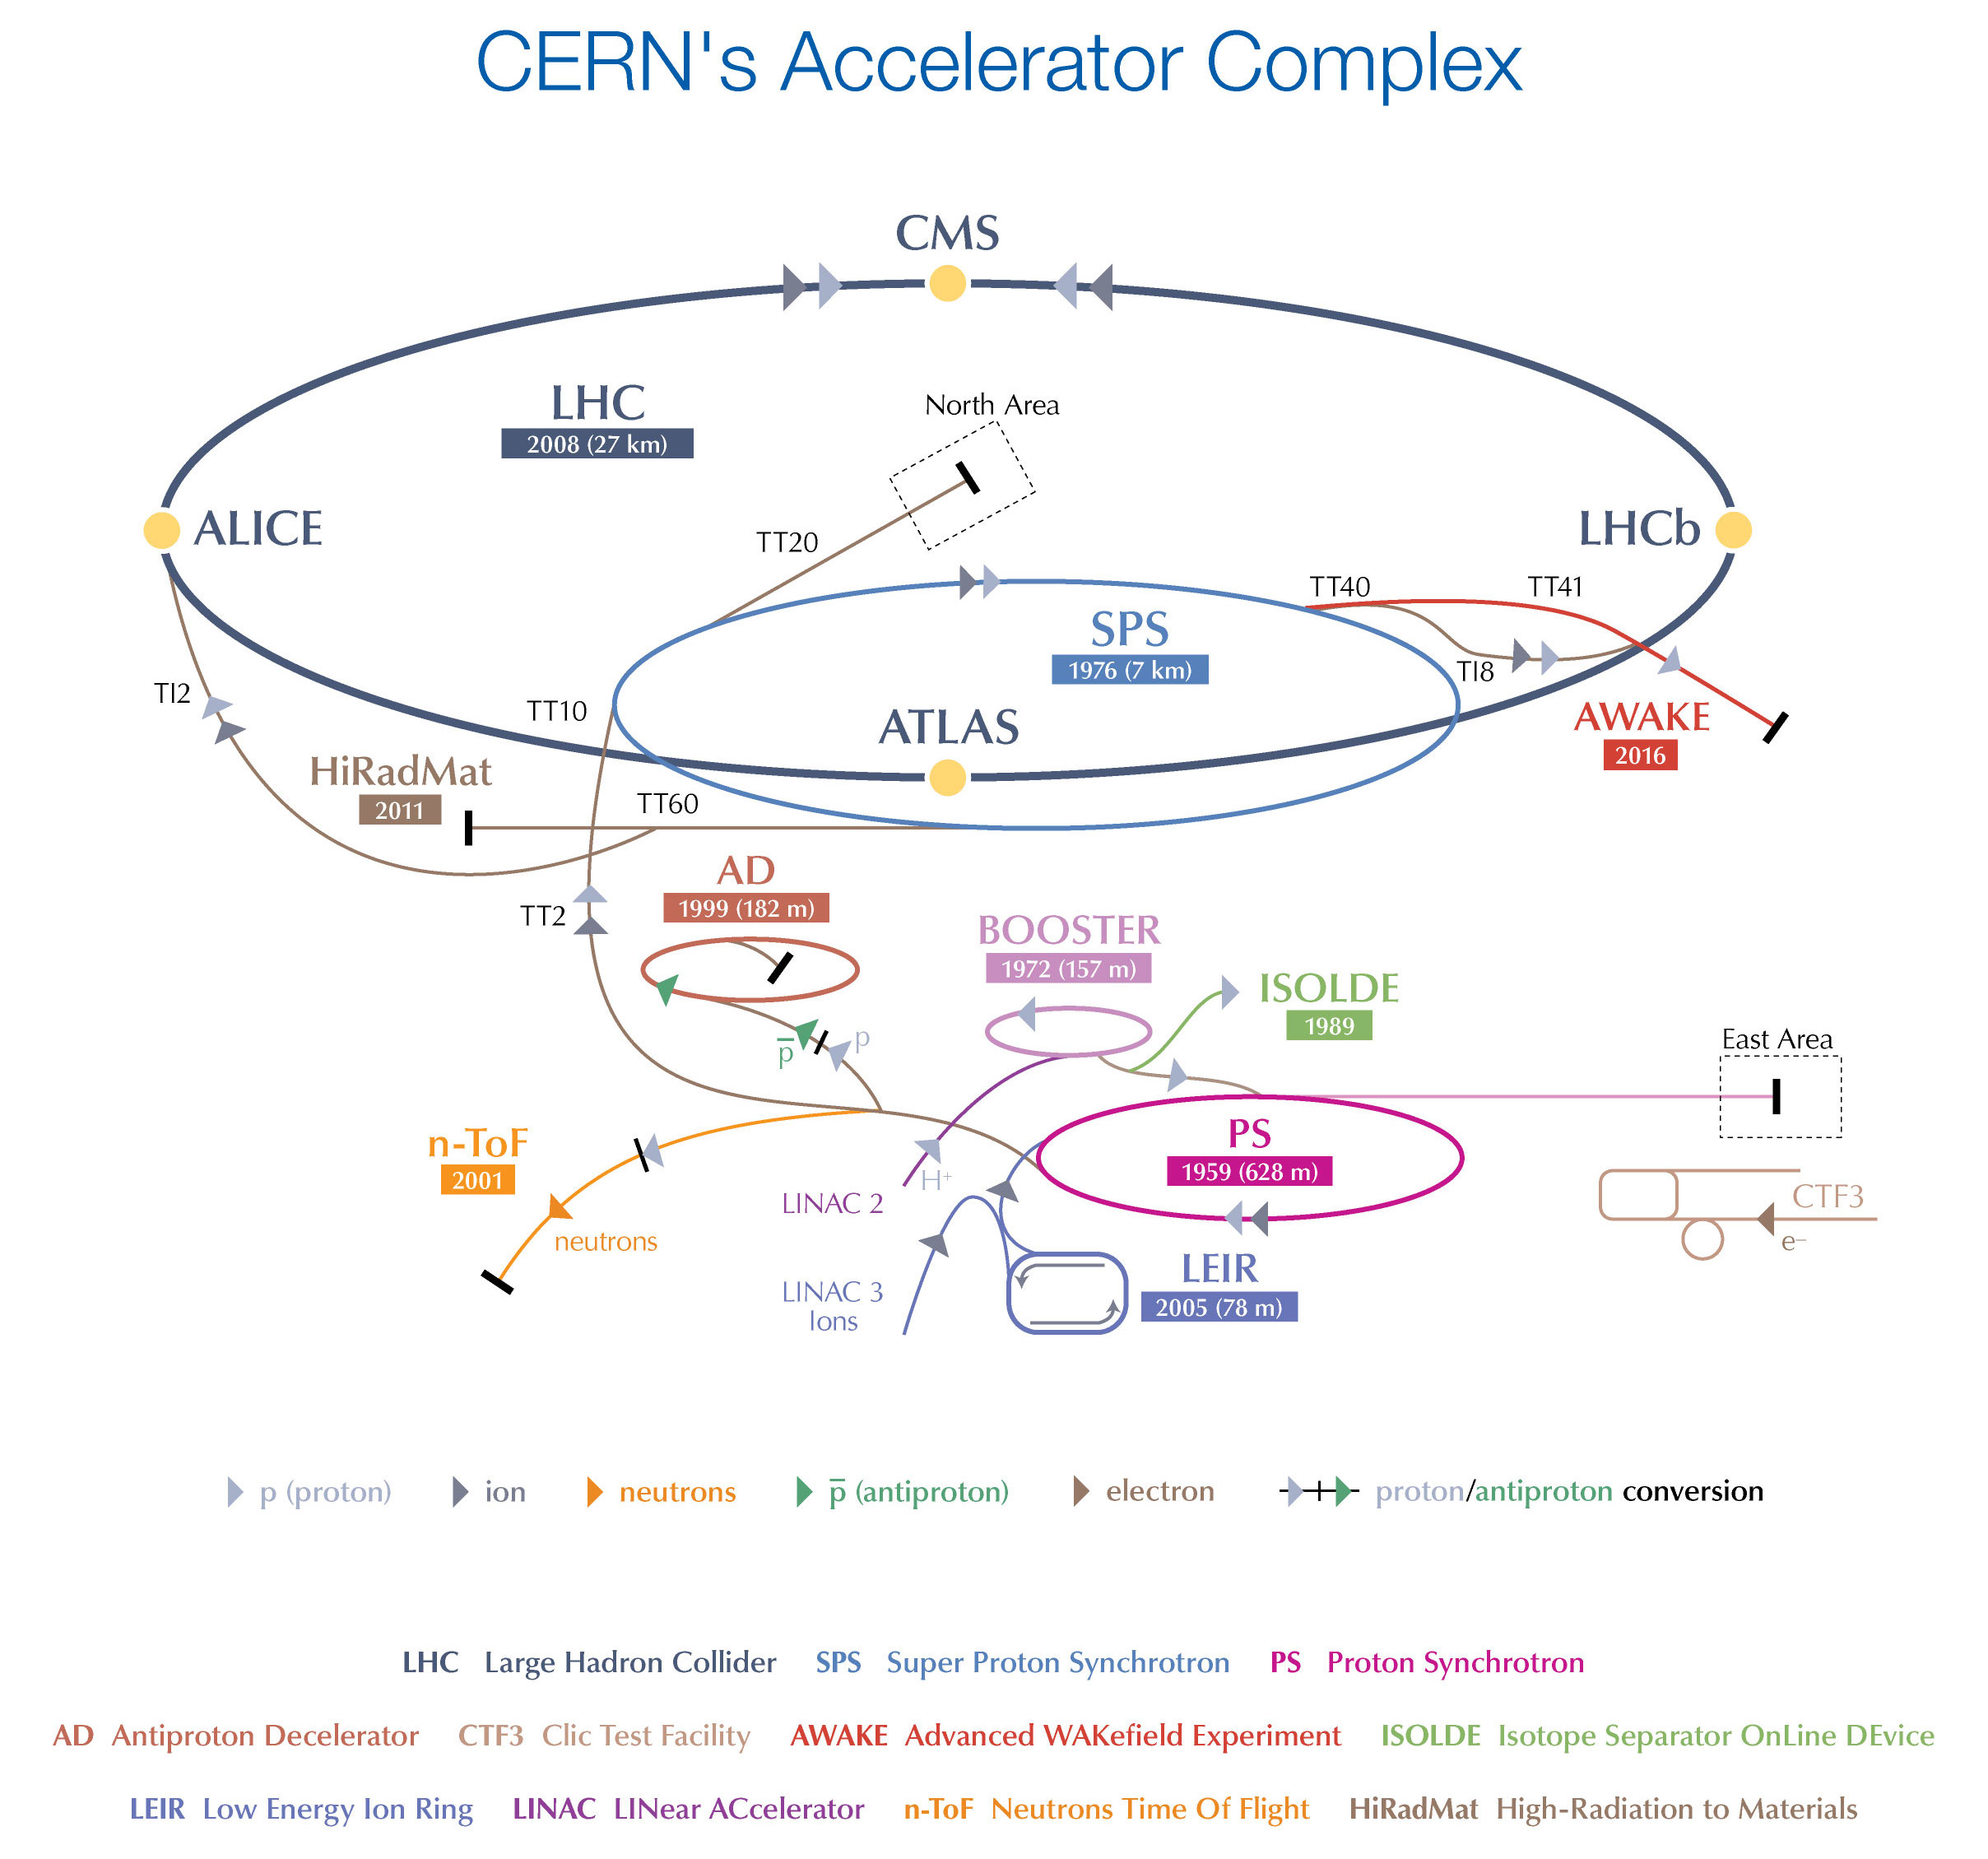
\includegraphics[width=0.9\textwidth]{Figures/CERNcomplex}
	\caption[The full CERN complex showing schematically the location of all the experiments on the ring complex, including the location of the four main experiments at the LHC: CMS, ATLAS, LHCb and ALICE.]{The full CERN complex showing schematically the location of all the experiments on the ring complex, including the location of the four main experiments at the LHC: CMS, ATLAS, LHCb and ALICE~\cite{CERNcomplex}. }
	\label{fig:CERNcomplex}
\end{figure}
% http://public-archive.web.cern.ch/public-archive/en/lhc/Facts-en.html

\section{The Large Hadron Collider}
\label{sec:LHC}

\subsection{A brief history of the LHC and CMS}
\label{ssec:LHCHist}
% TODO move ref
All dates from the LHC timeline are taken from~\cite{LHCtimeline}.
The first public announcement for the construction of the LHC was given on the 16th December 1994. 
A couple of years earlier, on the 1st October 1992, the CMS experiment submitted its letter of intent to the LHC Experiments Committee and on the 31st January 1997, the CMS experiment was approved.
Construction of the CMS site at Cessy began in July 1998, with the CMS cavern completed by the 1st February 2005.
In the following three years, the detector was assembled in segments above ground and lowered down into the cavern.
The final large detector segment was lowered on the 23rd July 2008.
The final dipole magnet of the LHC was lowered into place on 26th April 2007, heralding the completion of the full accelerator ring.
The 10th September 2008, was a very significant day in the history of the LHC marking the first circulation of proton beams around the collider. 
Shortly after, on the 19th, a fault occurred in an electrical connection between a dipole and quadrupole magnet, leading to a release of helium in the tunnels, causing significant damage to the LHC. 
In total 37 damaged magnets were replaced and 16 refurbished, with the final one being lowered on the 30th April 2009. 
Beams were present again in the machine on the 20th November 2009, over a year after the malfunction. 

Run I physics data collection at a centre-of-mass energy $\sqrts=7\TeV$, was started on the 30th March 2010 and ran through until the 18th October 2011. 
A second period of data collection at $\sqrts=8\TeV$ was performed from the 5th April 2012 to the 6th February 2013. 
During this time, enough data was collected to confirm the existence of a \SM{}-like \Hboson{} boson, officially announced on the 4th July 2012~\cite{CMS:Higgs}.
With one of the primary mandates of the LHC fulfilled, attention has turned to discovering the existence of physics beyond the \SM{} and measuring precisely the properties of the \Hboson{} boson and other \SM{} particles.

On the 3rd June 2015, after a two year long shutdown for upgrades, the collider started up again for Run II at an unprecedented $\sqrt{s}=13\TeV$. 
Four sets of data are scheduled to be taken during Run II, with a small set taken at the end of 2015 and major runs during 2016, 2017 and 2018.
Each major run lasts from a commissioning period around March to the end-of-year technical stop in December.
Run II data is scheduled to be collected until December 2018, from when it will enter a second long shutdown period before Run III scheduled to operate between 2020-2022.
This thesis uses the data set collected during 2016.

\subsection{Operating the LHC}
\label{ssec:LHCoperation}

The source for the proton beams is a small canister of hydrogen gas. 
The hydrogen gas is then ionised to create protons by applying a large electric field.
The collection of protons is then accelerated, within ultra-high vacuums, through the Linear Accelerator 2 (LINAC2), which uses alternatingly charged conductors to accelerate the bunch of protons up to an energy of 50\MeV{}, before being injected into the Proton Synchrotron Booster (PSB).
The PSB is an accelerator ring that boosts the protons to an energy of 1.4\GeV{} and passes them to the Proton Synchrotron (PS) which provides a further boost up to 25\GeV{}.
From the PS the proton bunches are accelerated in the Super Proton Synchrotron (SPS) to an energy of 450\GeV{}. 
The SPS splits the single beam into two counter-rotating ones and injects them into the LHC.
In the LHC, each proton beam can be accelerated up to a maximum energy of 7\TeV{} per beam. 
During Run I, this beam energy was operated at 3.5(4)\TeV{} and has been increased to 6.5\TeV{} for Run II. 

To reach these operational collision energies the proton bunches are accelerated, confined and squeezed by magnetic fields of up to 8.3\Tesla{} from over 9300 superconducting magnets. 
The most common type of magnet used in the LHC is the dipole magnet, of which there are 1232.
Each dipole magnet is 15\m{} long, weighs 35 tonnes and has a magnetic field strength of 8.3\Tesla{} which is used to bend the beam around the collider. 
Figure~\ref{fig:LHCdipole} shows a cross section through one of the LHC dipole magnets.
Each dipole contains two beam pipes for the counter-circulating beams and along each of these beam pipes are coiled niobium-titanium alloy wires which form the superconducting dipole magnet. 
Superconductivity in the magnet is achieved by a closed circuit of liquid helium, which cools the iron yoke to 1.9\Kelvin{}.
\begin{figure}[htpb]
	\centering
	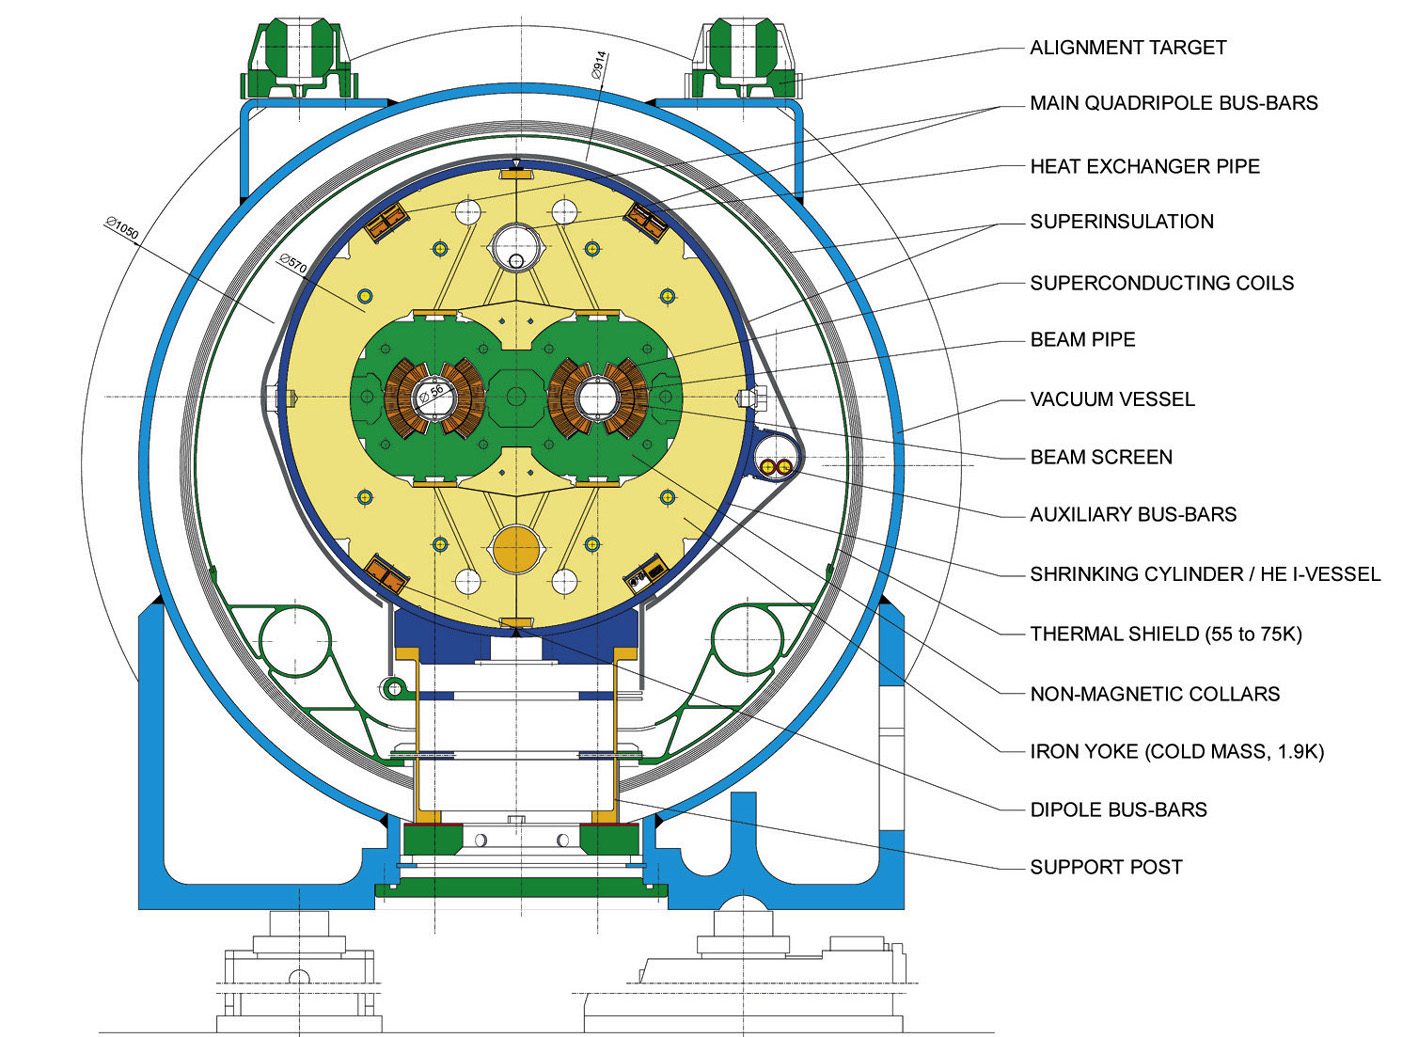
\includegraphics[width=0.8\textwidth]{Figures/LHCdipole}
	\caption[A cross section of a LHC dipole magnet.]{A cross section of a LHC dipole magnet~\cite{LHCdipolemagnet}. }
	\label{fig:LHCdipole}
\end{figure}
% Different specs for inner outer coils: http://lss.fnal.gov/archive/2015/conf/fermilab-conf-15-635-td.pdf
% Busbar = highvoltage power rail
% http://ieeexplore.ieee.org/stamp/stamp.jsp?arnumber=1211818

In addition to the dipole magnets, the LHC uses 858 quadrupole magnets. 
Of these, 392 are lattice quadrupoles used to stop the beam from defocussing over time due to the similarly charged beam constituents. 
Quadrupole magnets are also used to confine the proton beams as they are entering the experimental caverns. A set of three, known as an inner triplet, squeezes each beam to a diameter of 16\um{} to ensure a maximal number of collisions at the interaction point.
There are additional multipole magnets used to correct for other, smaller, effects present in the beam, such as the gravitational force on the protons. 
% electromagnetic interactions among bunches, electron clouds from the pipe wall

\section{Luminosity measurements}
\label{sec:lumi}

The instantaneous luminosity is defined as:
\begin{equation}
\label{eq:InsLumi}
\Lum = f \frac{n_{1}n_{2}}{4\pi \sigma_{x} \sigma_{y}}
\end{equation}
\Lum{} depends on the bunch crossing rate, $f$, the number of protons in each colliding bunch, $n_{1}$ and $n_{2}$, and the root-mean-square of the transverse beam sizes in the horizontal ($\sigma_{x}$) and vertical ($\sigma_{y}$) directions. 
The beams are assumed to have a Gaussian profile, of width $\sigma=16\um$, and to be colliding head-on.
For nominal running during Run II, each beam contains 3564 bunch spaces of which typically 2808 are filled during data taking, leading to a minimum bunch spacing of 25\ns{} and a collision rate $f=40\MHz$.
Each bunch contains $\approx 1.1\ten{11}$ protons, producing a peak $\Lum=1.50\ten{34}\Lunit$.
\Lum{} varies with respect to time due to the depletion of the protons in each bunch after every collision.
The decrease in luminosity is mitigated to a small extent by the reduction of the beam widths $\sigma_{x}$ and $\sigma_{y}$, however each beam has an approximate physics taking lifetime of ten hours before they need to be refilled.
The total number of inelastic collisions (known as minimum bias events) produced at the LHC, over a time $t$, can be estimated from the luminosity by:
\begin{equation}
\label{eq:nEvent}
\text{N} = \sigma_{\text{minbias}}\times\Lum_{\text{int}}, 
\end{equation}
where $\sigma_{\text{minbias}}$ is the minimum bias cross section.
$\Lum_{\text{int}}$ is the integrated instantaneous luminosity over time $t$
\begin{equation}
\label{eq:IntLumi}
\Lum_{\text{int}} = \int^{t}_{t_{0}}\Lum(t)\text{d}t.
\end{equation}
The $\Lum_{\text{int}}$ distribution during the 2016 data taking period is shown in the left panel of Fig.~\ref{fig:CMSLumi}, where a total of \Lumi{} of certified data was collected by the CMS experiment.
The right panel shows the delivered luminosity for all other years of data taking.
Using the current $\sigma_{\text{minbias}}$ measurement of 69.2\mb{}, this means that approximately $2.5\ten{15}$ collisions were processed in this period.
\begin{figure}[htpb!]
	\centering
	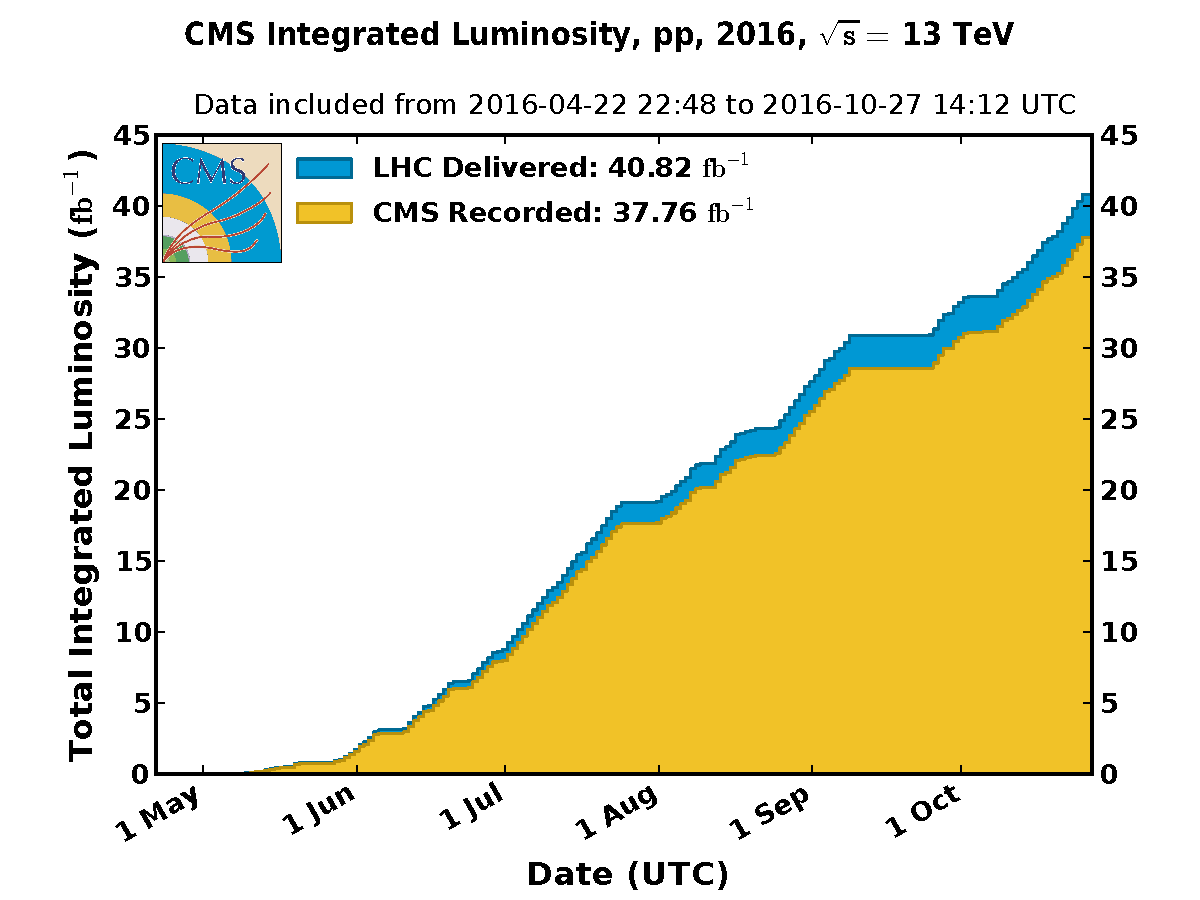
\includegraphics[width=0.49\textwidth]{Figures/LHC2016Lumi}
	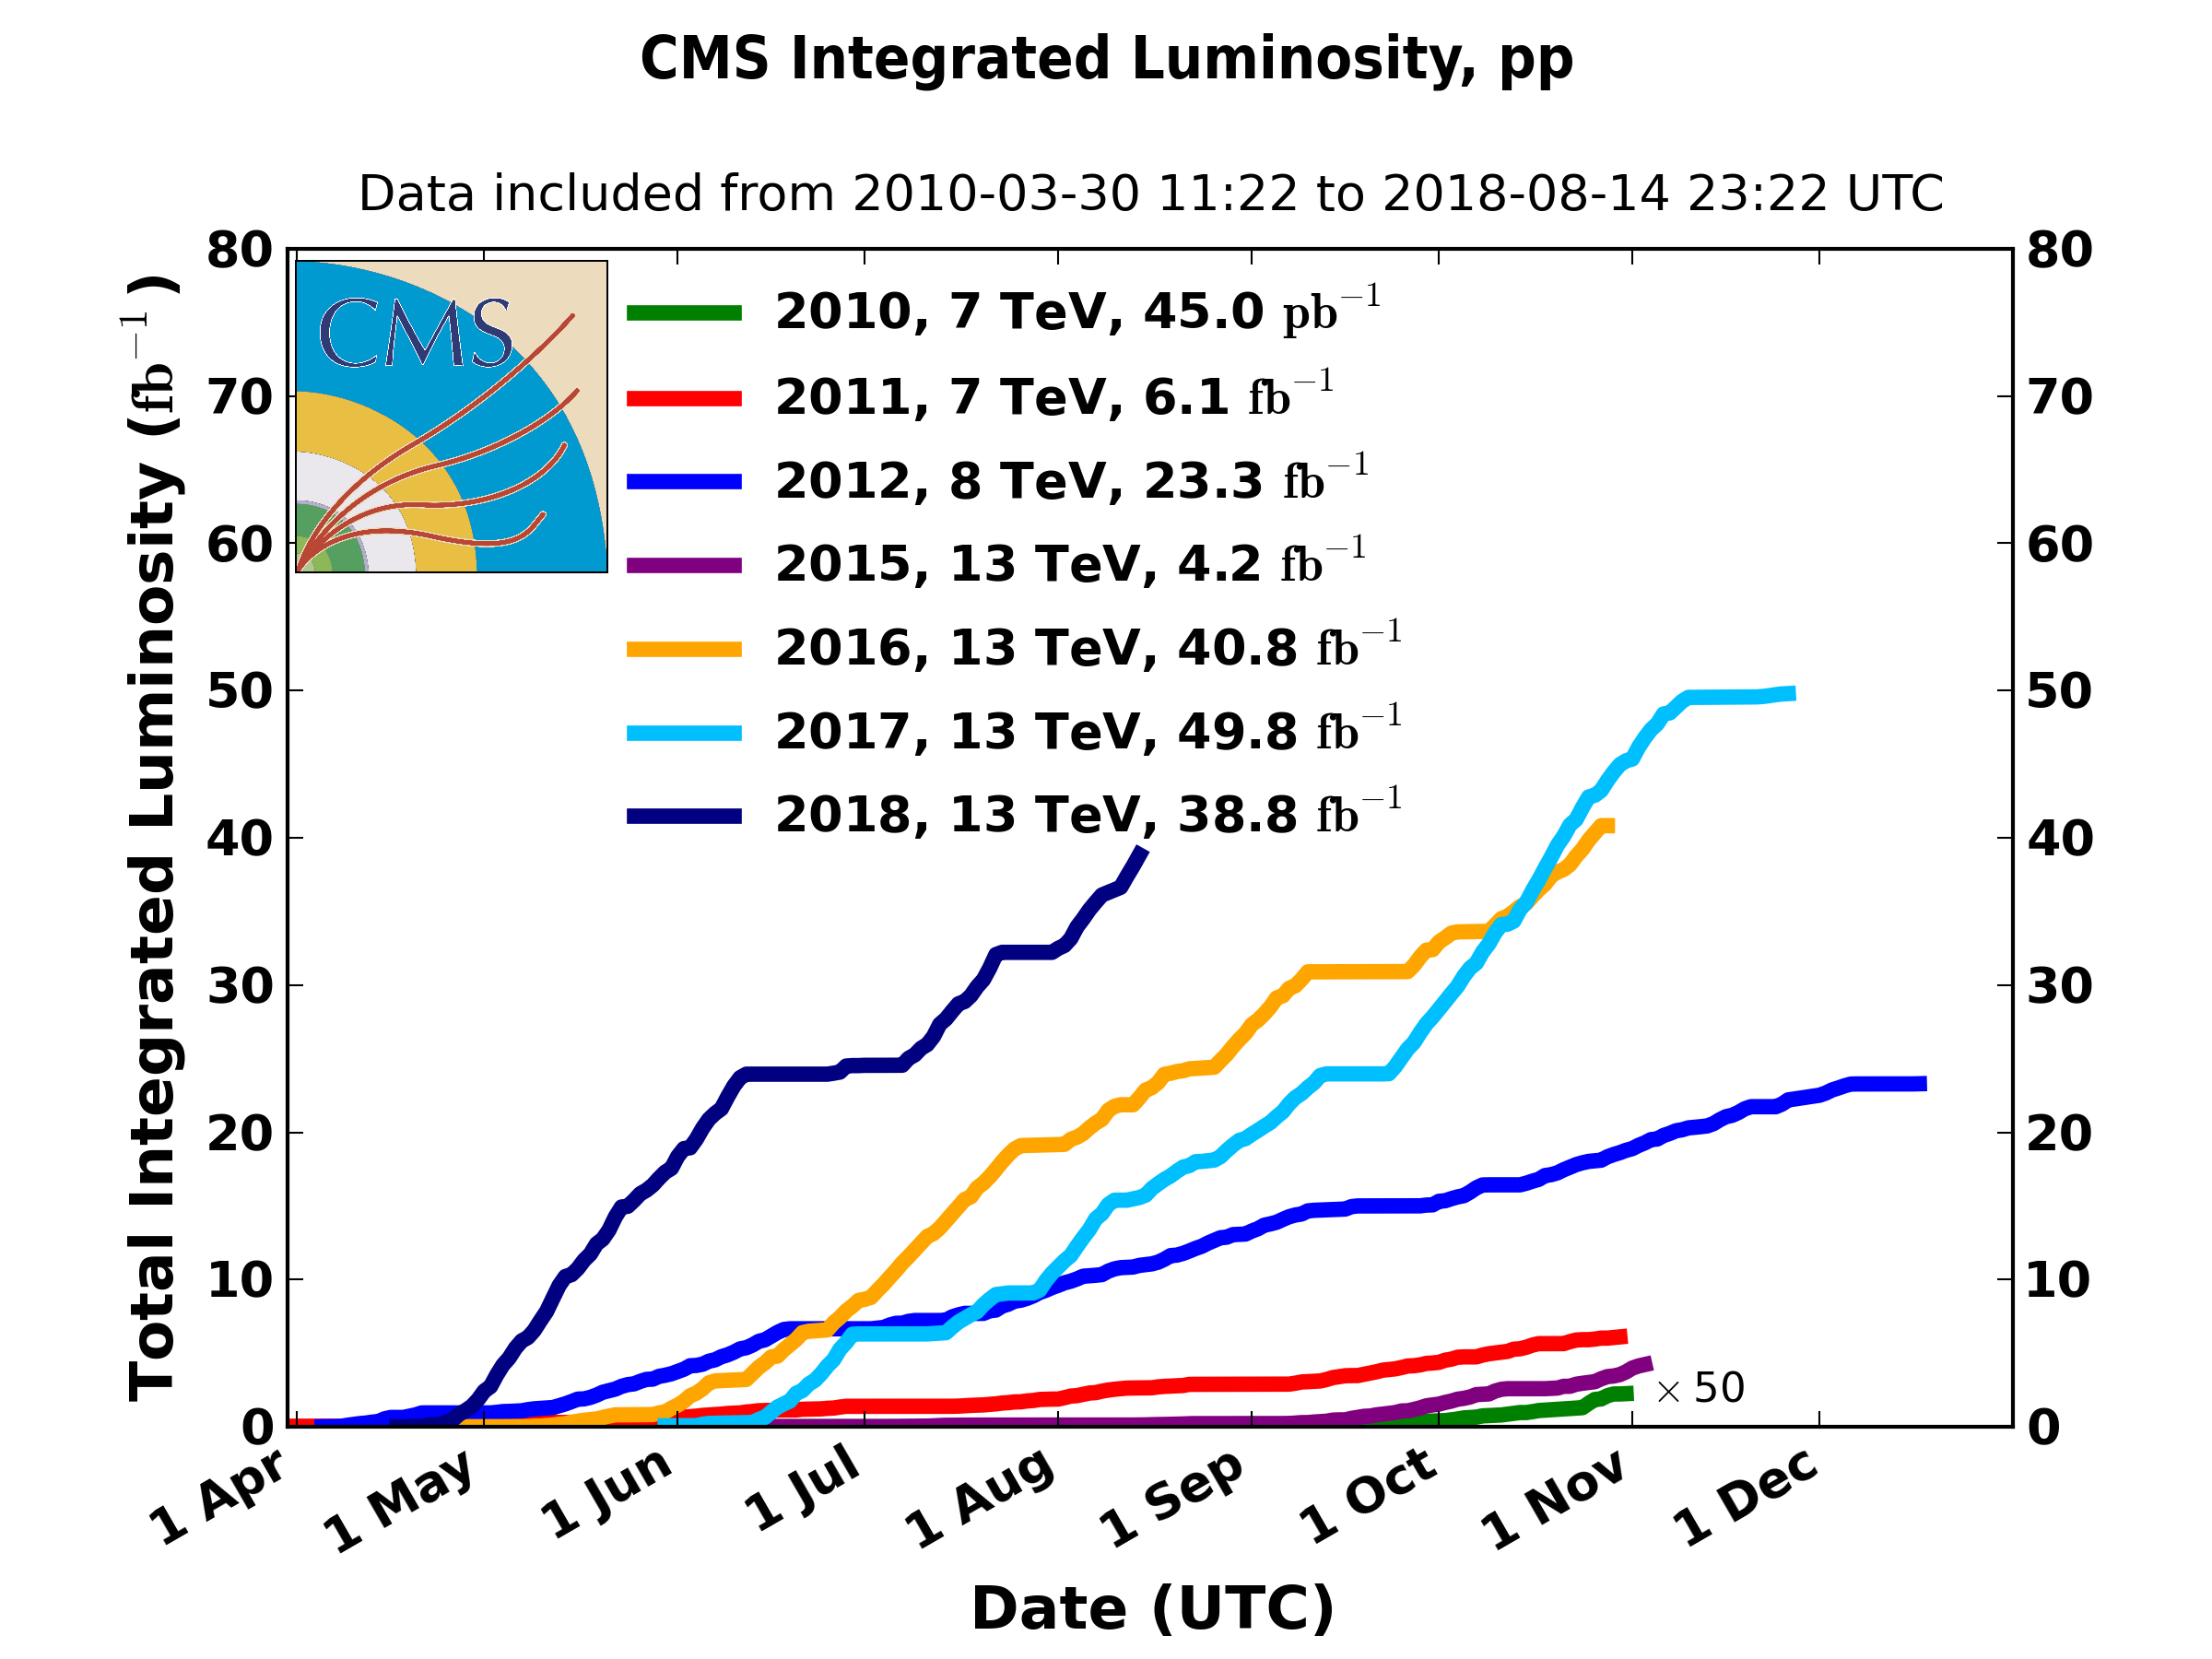
\includegraphics[width=0.49\textwidth]{Figures/LHCLumiAllYears}
	\caption[The left panel shows the delivered and recorded integrated luminosity during data taking in 2016 and the right panel the integrated luminosity delivered by the LHC for all years of operation.]{The left panel shows the delivered and recorded integrated luminosity during data taking in 2016 and the right panel the integrated luminosity delivered by the LHC for all years of operation. Figures taken from~\cite{CMS:CMSLumi}.}
	\label{fig:CMSLumi}
\end{figure}
More than one proton-proton interaction typically occurs in each bunch crossing and these additional interactions are referred to as \textit{in-time pileup}.
As the collision rate at the LHC is so high, it is also possible for remnants of previous bunch crossings to affect the current one, particularly in calorimeters where there is a latency higher than a typically bunch spacing.
These remnants are called \textit{out-of-time pileup}.
The average number of interactions per bunch crossing during 2016 data taking was approximately 30, as can be seen in Fig.~\ref{fig:CMSPU}, using a minimum bias cross section of $80\mb$.
Particles from pileup are included in the particle reconstruction of the event, leading to misidentification.
Reconstruction and pileup mitigation techniques are described in Secs.~\ref{ssub:antikt} and~\ref{sub:jet_energy_corrections}.
\begin{figure}[htpb]
	\centering
	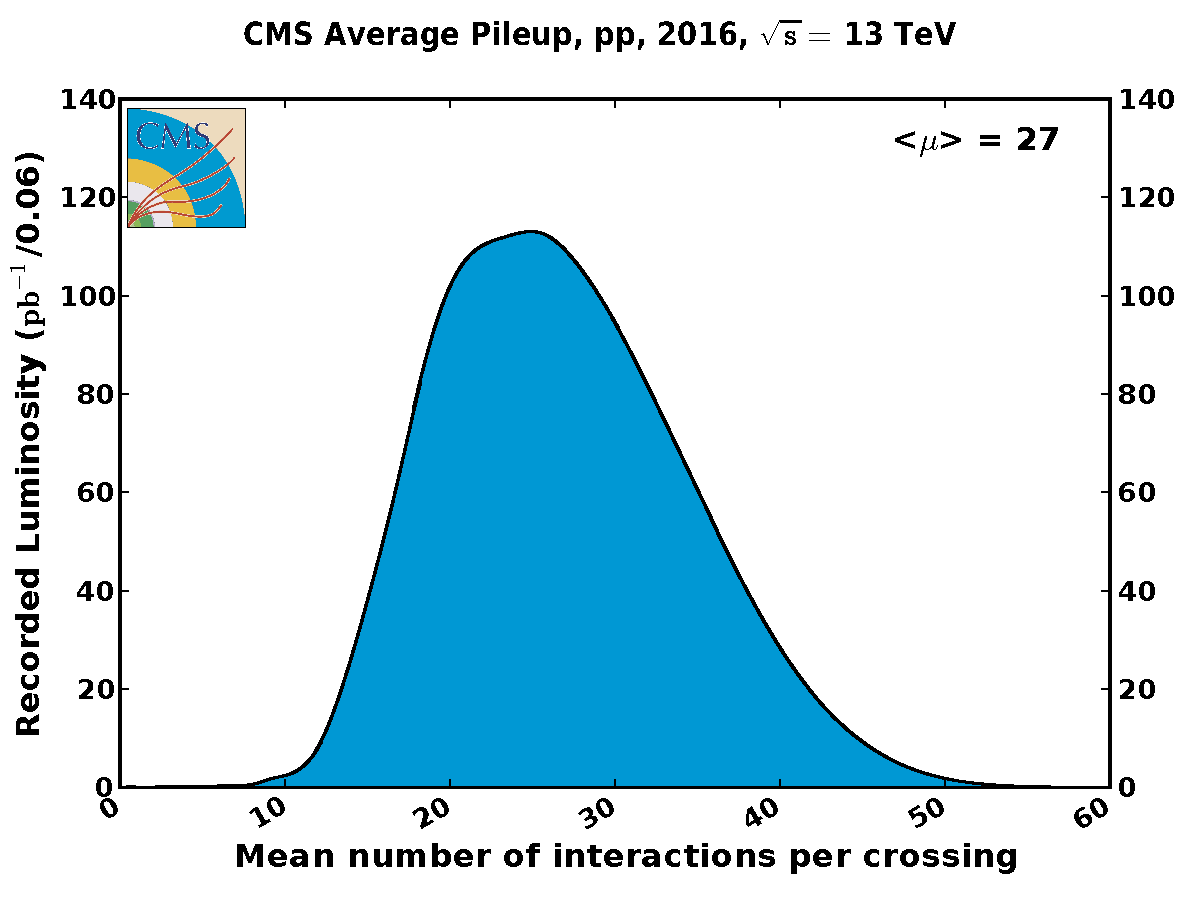
\includegraphics[width=0.6\textwidth]{Figures/CMSAvePU}
	\caption[The distribution of the number of interactions in a bunch crossing. The minimum bias cross section is taken to be $80\mb$.]{The distribution of the number of interactions in a bunch crossing. The minimum bias cross section is taken to be $80\mb$. Figure taken from~\cite{CMS:CMSLumi} }
	\label{fig:CMSPU}
\end{figure}

% sigma^2 (beam size) = epsilon.beta* (emittance . beta function)
% emittance – the spatial and angular spread of particles. A low emittance particle beam is a beam where the particles are confined to a small distance and have nearly the same momentum.
% Link to Tracker - lots of particles need high granularity tracker.
% Not quite head on collisions add another crossing angle factor
% 1.15 is design, 1.1 is actual http://accelconf.web.cern.ch/accelconf/hb2016/papers/moam5p50.pdf
% 27km / 3564b / 3e8 = 25ns :D
% Check

\section{The Compact Muon Solenoid}
\label{sec:CMS}

CMS is a general purpose detector, designed to be able to perform precision measurements of the standard model and searches for new physics~\cite{CMSExperiment}. 
It is a cylindrical, hermetic detector composed of a barrel region and two endcaps, each formed of layers of subdetectors around the beam collision point, as shown in Fig.~\ref{fig:CMSPicture}. 
These subdetectors, in order from the collision point, are the pixel and strip tracker, electromagnetic calorimeter (ECAL), hadronic calorimeter (HCAL) and muon chambers.
The superconducting magnet is situated in between the hadronic calorimeter and muon chambers.
To operate in a high luminosity environment the CMS experiment must have excellent resolution in each of its subdetectors and a low latency to manage the high collision rate. 
The materials used must be reliable while having maximal longevity when operating in a high-radiation environment.

CMS uses a right-handed coordinate system, where the $x$-axis points towards the centre of the accelerator ring, the $y$-axis points vertically upward and the positive $z$-axis lies parallel to the anti-clockwise beam axis. 
The azimuthal angle $\phi$, is measured from the $x$-axis in the transverse $x-y$ plane. 
The polar angle $\theta$, is measured from the positive $z$-axis in the $z-y$ plane.
At the CMS experiment, collisions are viewed in the centre-of-mass frame of the colliding protons, which means that the colliding partons usually have a Lorentz boost along the beam direction.
For this reason, the angles of the particles are normally expressed in terms of the rapidity ($y$) or pseudorapidity ($\eta$), in which the production is roughly constant.  
The rapidity is defined as
\begin{equation}
\label{eq:rap}
y\equiv {\frac{1}{2}}\ln\left({\frac{E+p_{z}}{E-p_{z}}}\right),
\end{equation}
where $E$ is the energy of a measured particle and $p_{z}$ is the $z$-component of the momentum.
Rapidity is advantageous to use as rapidity differences between two particles is invariant under a Lorentz boost along the $z$-axis.
At the LHC, most particles are highly relativistic such that the rest mass is small compared to the energy ($p_{z}\approx E\cos\theta$). This can be substituted into Eq.~\ref{eq:rap} and using trigonometric relations, the pseudorapidity is defined as
\begin{equation}
\label{eq:eta}
\eta \equiv -\ln\left(\tan\left({\frac{\theta}{2}}\right)\right).
\end{equation}

% Henceforth, angular measurements are given in terms of pseudorapidity.
Jet production in \pp{} collisions is roughly constant in $\eta$, reflecting the forward nature of the production.
The subdetectors at the CMS experiment extend to at least a pseudorapidity magnitude of 2.4, covering more than 95\% of the phase space. 
Individual subdetectors can extend to a higher $\abs{\eta}$, for example the forward detectors of the HCAL, to study very boosted jets or the underlying event.
The acceptance within $\abs{\eta} < 2.4$ can be hampered by issues such as the gap between barrel and endcap detectors.
% 2.4 => 10deg. 1 str=33 deg. lost=0.61str. pc = 4.8

To completely describe the kinematic properties of a particle, its energy and momentum must be known. 
While it is not possible to detect the complete momenta spectrum of an event, due to many particles produced in the collision being lost down the beam pipe and the unknown boost of the partons, it is possible to measure the momenta in the transverse plane, where the sum of the momenta is conserved. 
To measure the transverse momenta and energy of particles, CMS uses a combination of hits in the tracking systems from charged particles and energy deposits in the calorimeters.
These subsystems are described in more detail in the following sections.

% \begin{landscape}
% \centering
\begin{figure*}[htpb]
	\centering
	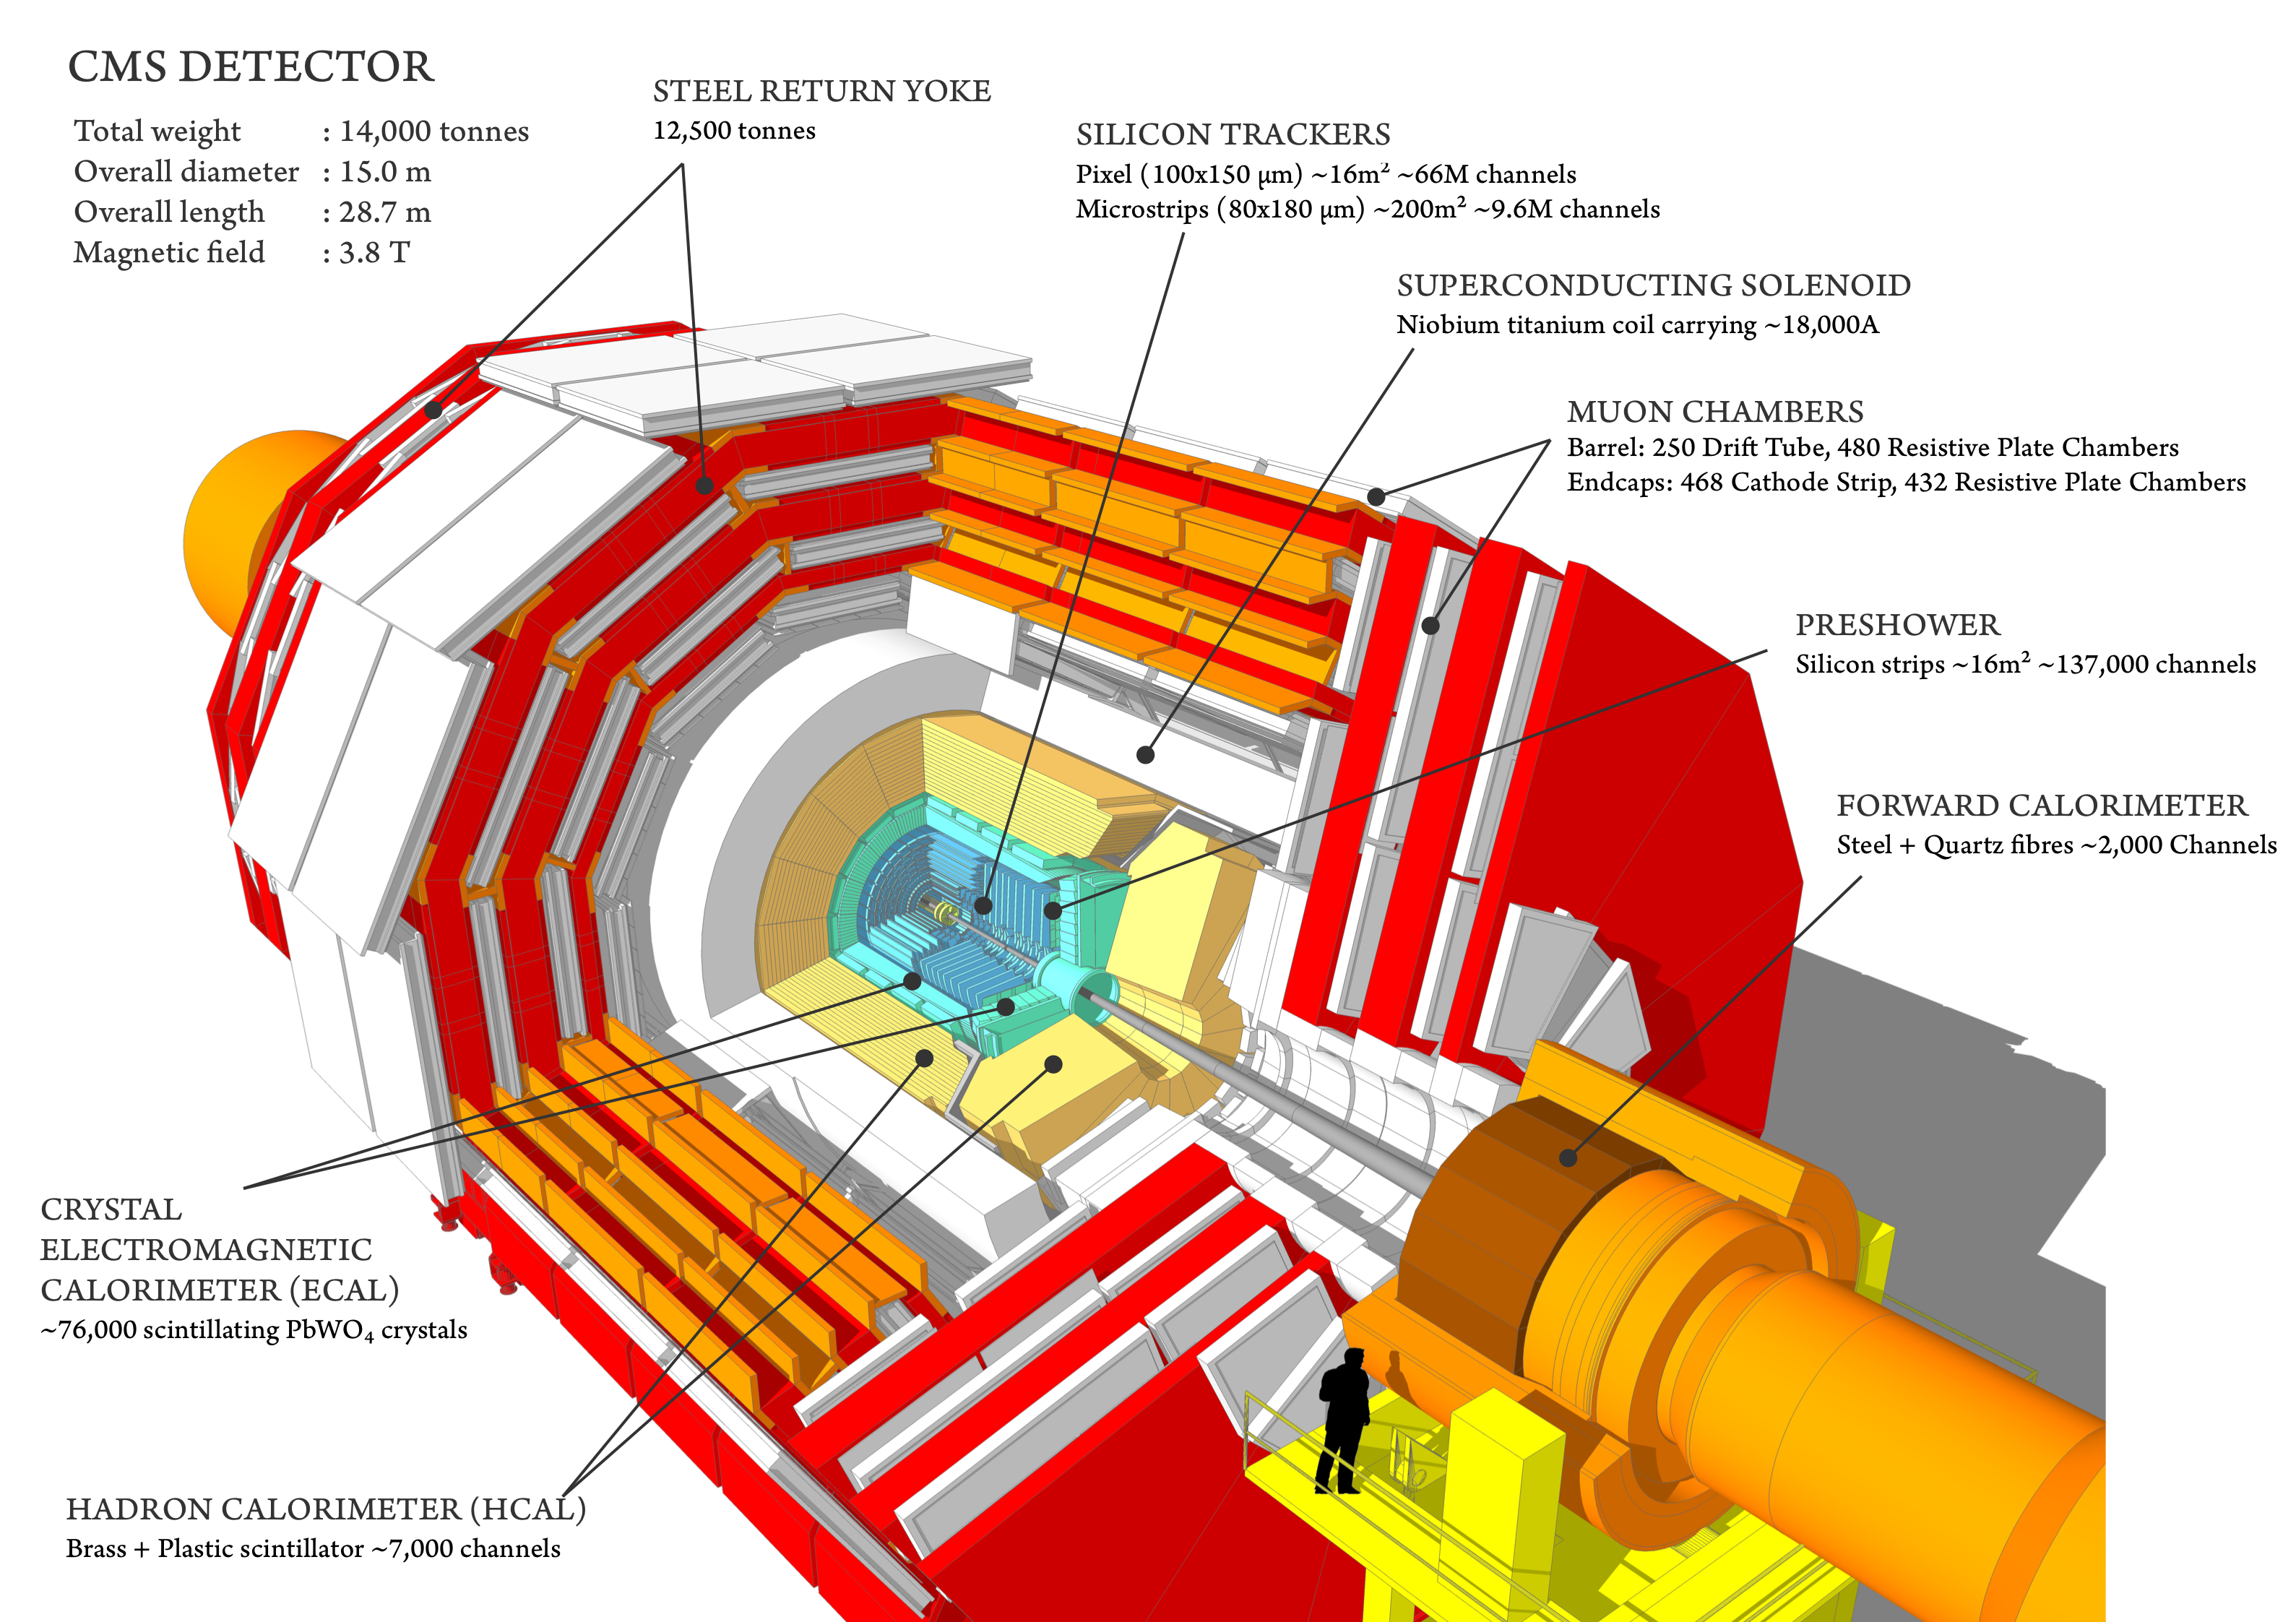
\includegraphics[width=\linewidth]{Figures/CMSPicture}
	\caption[A schematic of CMS, sliced to show the internal layout. It consists of layers around the central interaction point in the order of silicon pixel and strip detectors, electromagnetic and hadronic calorimeters, superconducting magnet and finally muon chambers. ]{A schematic of CMS, sliced to show the internal layout. It consists of layers around the central interaction point in the order of silicon pixel and strip detectors, electromagnetic and hadronic calorimeters, superconducting magnet and finally muon chambers~\cite{CMSPicture}.}
	\label{fig:CMSPicture}
\end{figure*}
% \end{landscape}

\subsection{CMS pixel and strip trackers}
\label{ssec:Tracker}
% Page 62

Figure~\ref{fig:CMSTracker} shows the layout of the silicon tracking detectors in CMS. 
Closest to the interaction point are the pixel detectors consisting of three barrel layers situated at radial distance $r=4.4, 7.3$ and 10.2\cm{} in the transverse plane from the interaction point with two endcap disks lying at $z=\pm34.5$ and $\pm46.5\cm$.  
There are 65 million pixels in the inner tracker, each $100\times150\umsq$, giving a total active area of 1.06\msq{}.
Surrounding the pixel detectors are the silicon strip tracker sensors. 
These are arranged into four subsystems: the Tracker Inner Barrel and Disks (TIB and TID), the Tracker Outer Barrel (TOB) and the Tracker Endcaps (TEC).
The TIB consists of four barrel layers between $20<r<55\cm$ with each end capped by 3 disks ($|z|<118\cm$) forming the TID. 
Wrapping around the TIB and TID, is the TOB consisting of six barrel layers between $55<r<116\cm$. 
Finally, the TEC consist of nine disks between $124<|z|<282\cm$, capping the TIB, TID and TOB.
There are $15\,148$ silicon strip modules in total that make up the outer tracker, giving a total active surface area of 198\msq{}. 
Some strip layers in the tracker, coloured blue in Fig.~\ref{fig:CMSTracker}, have back-to-back modules, rotated with respect to each other by a small stereo angle ($\approx5\de$) in order to improve the 3-dimensional point resolution by providing a measurement of the $z$ co-ordinate in the barrel and $r$ in the disks.

\begin{figure}[htpb]
	\centering
	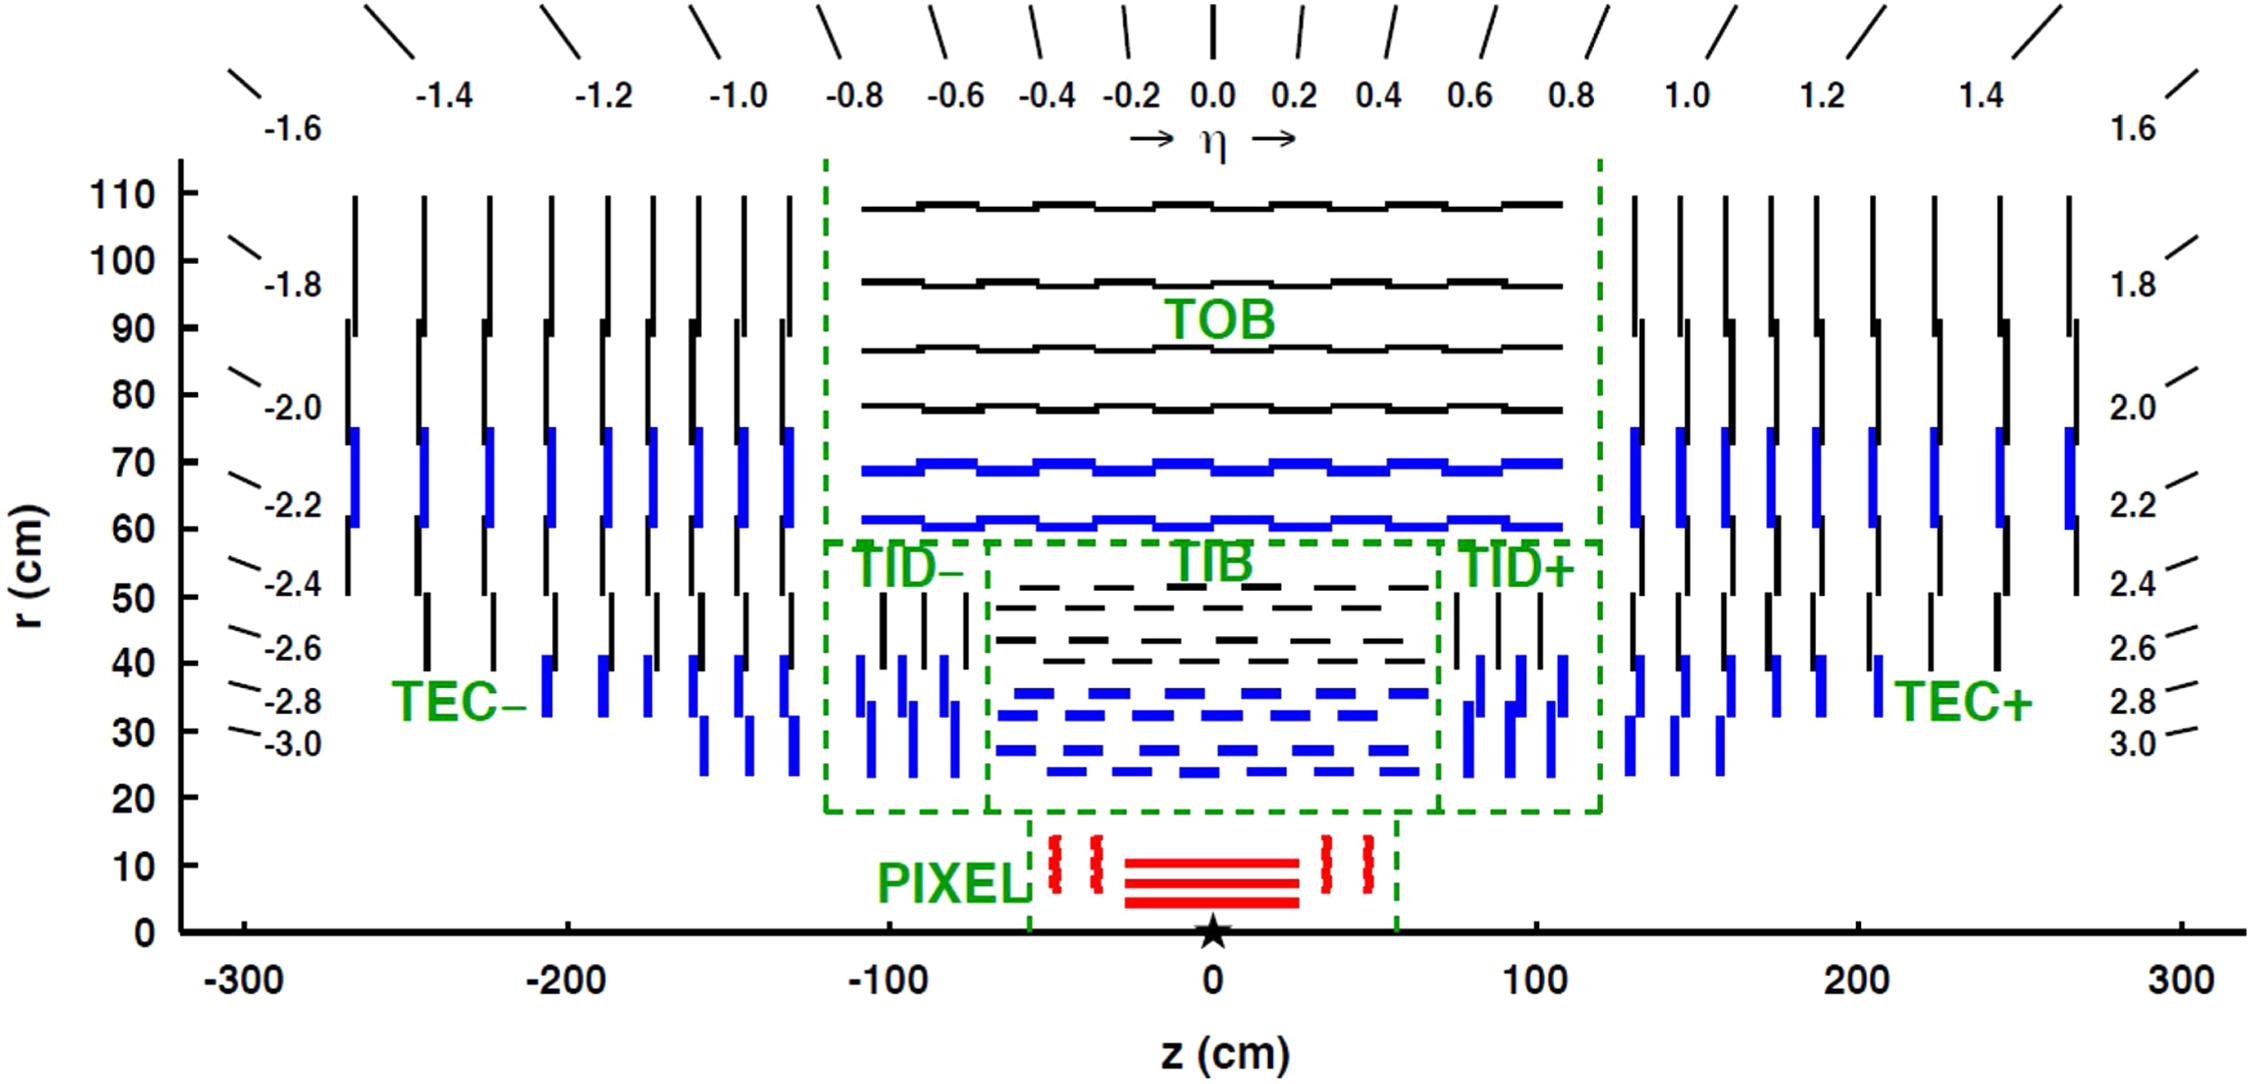
\includegraphics[width=\textwidth]{Figures/CMSTracker2.jpg}
	\caption[A slice through the CMS tracker detector in the $r-z$ plane. The separate subsystem regions have been highlighted and are classified as the Tracker Inner Barrel and Disks (TIB and TID), the Tracker Outer Barrel (TOB) and the Tracker Endcaps (TEC). The Pixel subsystem is highlighted in red. Back-to-back stereo strip modules are highlighted in blue.]{A slice through the CMS tracker detector in the $r-z$ plane. The separate subsystem regions have been highlighted and are classified as the Tracker Inner Barrel and Disks (TIB and TID), the Tracker Outer Barrel (TOB) and the Tracker Endcaps (TEC). The Pixel subsystem is highlighted in red. Back-to-back stereo strip modules are highlighted in blue. Figure taken from~\cite{CMSTrackerPerformance}.}
	\label{fig:CMSTracker}
\end{figure}
% of size $100\times150$ $\mu m^{2}$, uses 

Each tracking sensor operates in a similar manner.
For the pixel sensors, an \nnjunc{} junction is utilised where the silicon has been doped with phosphorous to different degrees. 
For the strip sensors, a \pnjunc{} junction is used where a silicon strip doped with boron has been laid on the bulk n-type silicon.
Doping with phosphorous causes the silicon to become an electron donor (n-type) and doping with boron to become an electron acceptor (p-type).
The n(p)$^{+}$-type silicon is where silicon has been doped to such an extent that the resistivity is very low.% resulting in a very good chip readout connection.

In the case of the silicon strip sensor, electrons diffuse from the bulk n-type silicon to a strip of p$^{+}$-type silicon, creating a small opposing electric field from the formation of ions either side of the \pnjunc{} junction.
The field stops further electron-hole movement and forms a potential step.
The region with no excess electrons or holes is known as the depletion zone, which causes the junction to act as a diode.
A reverse bias voltage is applied to ensure the silicon is fully depleted by attracting the free electrons and holes away from the \pnjunc{} junction.
% A reverse bias voltage is applied to counteract this electric field, increasing the size of the stable depletion zone.
% The reverse bias voltage causes the p$^{+}$-type silicon strip to act as a diode, cutting any... TODO.
When a charged particle ionises the n-type bulk silicon, the electrons and holes produced ($\approx 30\,000$) drift in the large electric field such that the holes move towards the p$^{+}$-type silicon producing a small signal current which is then amplified and shaped.
This method can be applied to any semiconductor junction where each side has different doping concentrations.

% http://ieeexplore.ieee.org/stamp/stamp.jsp?arnumber=4774788
The pixel detector receives a charged particle flux of $1\MHz\mmsqinv$. 
At this high rate of particles the pixels must have a high granularity to keep the fraction of channels hit (occupancy) reasonable.
A low occupancy in the pixel detector is necessary to reconstruct individual particle tracks back to an interaction vertex, in a high-track environment.
Lower occupancies present in the TOB and TEC mean that a longer strip can be used, however this incurs an increase in noise, which is alleviated by increasing the thickness of the silicon sensor from 320\um{} to 500\um{}.
Tracks reconstructed in the pixel and strip detectors can then be used in vertex reconstruction, particle identification and charged particle momenta measurements.
The track reconstruction is detailed in Sec.~\ref{sub:Particle_flow_elements}.
% TODO APV
% TODO Endcap turbine shape - due to Lorentz drift in non uniform magnetic field.

% Both the pixel and tracker use the same bulk silicon.

% A total of TODO sensors are used in the pixel and tracker...
% The electrons and holes drift in opposite directions due to a TODOkV applied electric field (TODO the bias voltage).
% The current created by the electrons and holes is readout from the sensor
% p = Nholes, n = nElectrons
% https://cds.cern.ch/record/2282804/files/thesis.pdf


% pn junction - depletion zone holes <--> electrons. Creates small electric field opposing further drift and diffusion. Stable area. Made bigger or smaller by applying Pot Diff. Forward bias is smaller DZ, Rear Biased is larger. Want larger... -> low leakage current. Charged particle passes leaving 30000eh pairs
% https://www.hephy.at/fileadmin/user_upload/Halbleiterdetektoren.pdf

% \subsubsection{New Pixel Detector}
% \label{sssec:Tracker}
% Include the new 2017 Pixel detector?

\subsection{Electromagnetic calorimeter}
\label{ssec:ECAL}
% http://cms.web.cern.ch/news/crystal-calorimeter
% https://arxiv.org/pdf/1306.2016.pdf
% Moliere Radius: The radius of a cyclinder which contains 90% of the EM showers energy deposition. Smaller Moliere radii mean better shower spatial resolution and better shower separation due to smaller degree shower overlaps.
% Radiation Length: 

The CMS ECAL, as shown in Fig.~\ref{fig:CMSECAL}, is made of three subsystems: the barrel, the endcaps and the preshower detector.
Together, they form a compact coverage around the interaction point, up to $\abseta<3$.
\begin{figure}[htpb]
	\centering
	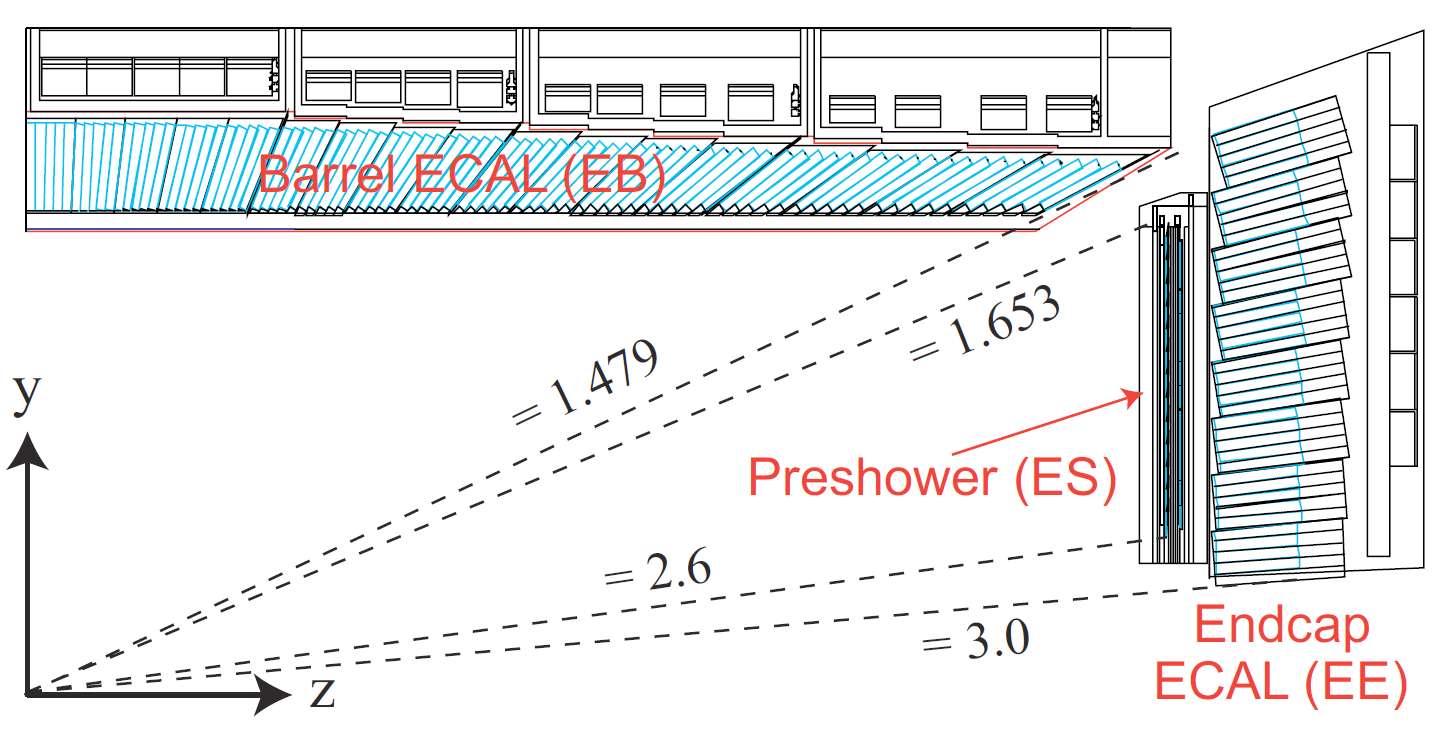
\includegraphics[width=\textwidth]{Figures/CMSECAL2}
	\caption[A geometrical quarter view of the CMS ECAL, highlighting the barrel, endcap and preshower detector regions.]{A geometrical quarter view of the CMS ECAL, highlighting the barrel, endcap and preshower detector regions. Figure taken from~\cite{CMSTDRV1}.}
	\label{fig:CMSECAL}
\end{figure}
% http://cms-project-ecal-p5.web.cern.ch/cms-project-ECAL-P5/approved/detector.htm
A total of $75\,848$ lead tungstate (\PbWO{}) scintillating crystals are used in the ECAL barrel and endcaps.
In the barrel section, the crystals are laid out in an $\eta-\phi$ grid extending to $\abseta<1.479$.
The inner surface of the barrel is at $r=1.29\m$, with each crystal having a front surface area of $2.2\times2.2\cmsq$ and length 23\cm{}.
In each endcap, the crystals are instead laid out in a $x-y$ grid, with the front surfaces at $z=\pm 3.14\m$, extending through $1.479 < \abseta < 3.0$. 
Each endcap crystal has a front surface area of $2.9\times2.9\cmsq$ and a length of 22\cm{}.
All the crystals are slightly off-centre with respect to the primary interaction point to avoid particles being lost down the small gaps between adjacent crystals.

\PbWO{} is an ideal choice for the CMS ECAL due to its short radiation and Moli\`ere lengths of 0.89 and 2.2\cm{} respectively. 
The radiation length gives a measure of the penetration of the EM shower into the crystal and the Moli\`ere length how confined the EM shower is, such that a cascade will mostly be contained within one crystal. 
In addition, \PbWO{} crystals are very fast with 80\% of the blue-green scintillation light being emitted in the time it takes for another collision to occur.
The light emission from the \PbWO{} crystals is relatively small at 30\photon{} per\MeV{} of energy deposited and therefore needs to be amplified using silicon avalanche photodiodes (barrel) and vacuum phototriodes (endcaps).
\PbWO{} is also radiation resistant tolerating up to $6.2\ten{17}\MeV\pow{kg}{-1}$ of radiation energy.
% 0.1\unit{MGy}.
% 0.1MGy = 100000 joule/kg
% What the hell are the APD and VPT and how do they work?
% 1 Gray = one joule of radiation energy per kilogram of matter

The purpose of the ECAL preshower detector is to distinguish between a high energy single photon and a $\pi^{0}$ decaying into two closely spaced photons.
To do this the preshower consists of two layers of lead, which initiate an electromagnetic shower for photons (and electrons), each closely followed by a layer of silicon strip detectors. 
The silicon strips are placed orthogonal to each other to measure shower positions precisely and are fine enough in granularity to differentiate between a single photon shower and multiple close-spaced photons.
A $\pi^{0}$ decaying in the barrel typically has low enough energy not to need the additional resolution provided by the preshower detector. 
The preshower degrades the resolution of the ECAL endcap due to the dense lead plates, however as the energy deposited within the lead is proportional to that deposited in the silicon, a correction can be applied mitigating the effect.
% http://www.hephy.at/project/cms/trigger/globalTrigger/trans/MEDIEN/Publications/CMSBooklet/Info_for_CMSBooklet/PreshowerFAQ_files/CMS3d.html

These attributes mean that the ECAL can be both compact enough to fit within the magnet and granular enough to perform with high energy resolution.
The resolution performance is measured by fitting a Gaussian function to the reconstructed energy distributions at different test beam energies and is parametrised by
\begin{equation} \label{eq:ECALRes}
	\left(\frac{\sigma_{\mathrm{ECAL}}}{E}\right)^{2} = \left(\frac{S}{\sqrt{E}}\right)^{2} + \left(\frac{N}{E}\right)^{2} + C^{2},
\end{equation}
where $S$ is a stochastic term (number of photoelectrons), $N$ is a noise term (electronics and digitisation) and $C$ is a constant term (leakage from the back of the ECAL).
% stochastic: having a random probability distribution or pattern that may be analysed statistically but may not be predicted precisely.
% S: statistical based, photoelectrons
% N: electronics. digitization
% C: leakage, nonuniformities in crystal
The left panel of Fig.~\ref{fig:CMSECALRes} shows the energy resolution with respect to the energy deposited in a $3\times3$ crystal lattice around incident electrons at a test beam measurement before the beginning of Run I with the values for $S$, $N$ and $C$ shown. 
The right panel shows the energy resolution with respect to $\abs{\eta}$ from the most recent public measurement~\cite{CMSECALRESMEAS}.
It is extracted from an unbinned likelihood fit on $Z\rightarrow e^{+}e^{-}$ events collected in 2015 for electrons with low brehmstrahlung radiation and $\ET\approx45\GeV$.
The resolution was measured to be $<2\%$ for $\abseta<1.0$ and between $2-5\%$ elsewhere.
\begin{figure}[hpb!]
	\centering
	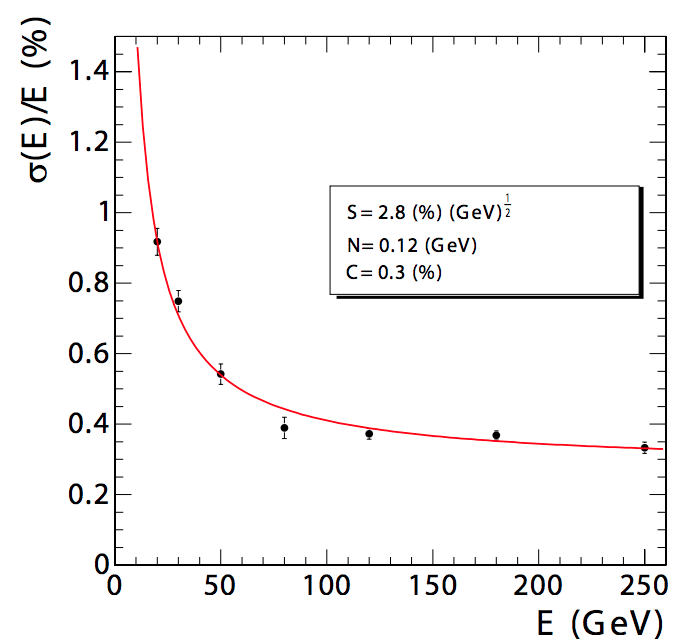
\includegraphics[width=0.6\textwidth]{Figures/CMSECALRES} \\
	\vspace{2cm}
	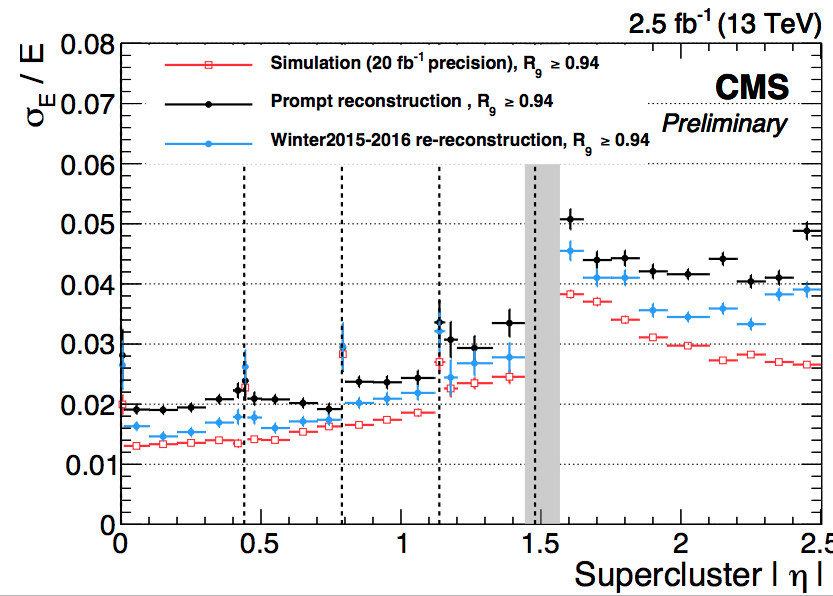
\includegraphics[width=0.8\textwidth]{Figures/CMSECALRES2}
	\caption[The upper panel shows the energy resolution of the CMS ECAL measured in a beam test. The energy was measured in a $3\times3$ crystal lattice with the electron striking the central crystal. The lower panel shows the resolution extracted from an unbinned likelihood fit on $Z\rightarrow e^+e^-$ events.]{The upper panel shows the energy resolution of the CMS ECAL measured in a beam test. The energy was measured in a $3\times3$ crystal lattice with the electron striking the central crystal. The lower panel shows the resolution extracted from an unbinned likelihood fit on $Z\rightarrow e^+e^-$ events. Figures taken from~\cite{CMSExperiment, CMSECALRESMEAS}.}
	\label{fig:CMSECALRes}
\end{figure}
% Not public measurements at 13TeV?

% 61200 in the barrel, 7324 in each endcap 
% Each crytal covers 0.0174 (1deg) in phi and eta.
% Actually 2.86 cm.
% Barrel is structured as 36 identical “supermodules,” each covering half the barrel length and corresponding to a pseudorapidity interval of 0 < |η| < 1.479. The crystals are quasi-projective (the axes are tilted at 3◦ with respect to the line from the nominal vertex position) ∆η. 
% The endcaps (EE), at a distance of 314 cm from the vertex and covering a pseudorapidity range of 1.479 < |η| < 3.0, are each structured as 2 “Dees”, consisting of semi-circular aluminium plates from which are cantilevered structural units of 5×5 crystals, known as “supercrystals.”


\subsection{Hadronic calorimeter}
\label{ssec:HCAL}
% The \MET can be inferred from all the deposits in the HCAL combined with all the deposits the ECAL.
The majority of the hadronic calorimeter, shown in Fig.~\ref{fig:CMSHCAL}, sits within the superconducting solenoid. 
It contains sampling calorimeters in the barrel (HB) and in the two endcaps (HE). 
The HB operates to an $\abseta<1.4$ and the HE covers the range to $1.4<\abseta<3.0$.
The HB is radially restricted between the ECAL and the superconducting magnet at $1.77\m < r < 2.95\m$ and as such there is only a limited amount of absorber present necessitating the requirement for scintillator plates situated outside the solenoid (HO).
The HB is divided into two half-barrels each composed of 18 identical azimuthal wedges consisting of alternating layers of non-magnetic, short radiation-length brass absorber and plastic scintillator tiles.
Each wedge is capped by steel absorber for structural strength.
The HE are formed of a similar structure.
Around $70\,000$ scintillating tiles of dimensions $\Delta\eta\times\Delta\Phi=0.087\times0.087$ for $\abs{\eta}<1.6$ and $0.17\times0.17$ for $\abs{\eta}>1.6$ are used in the construction of the HCAL.

The forward hadronic detectors (HF) are situated $\pm11.2\m$ from the primary interaction point within a pseudorapidity range of $3.0<\abseta<5.2$.
The HF, which is very close to the beam line, receives a large flux of particles and therefore must be very radiation resistant.
To this end it is made of steel and quartz fibres, where the emitted Cherenkov light in the quartz fibres is passed to photomultipliers and read as signal~\cite{HF}.
The HF allows for the reconstruction of forward jets and also allows for a better description of \ptmiss{}.

\begin{figure}[htpb]
	\centering
	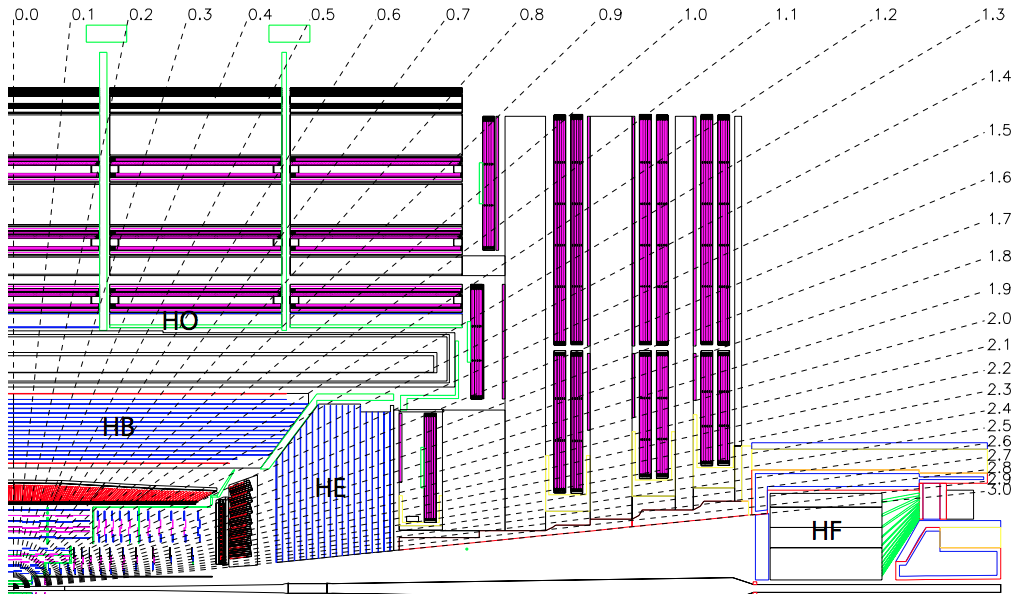
\includegraphics[width=\textwidth]{Figures/CMSHCAL}
	\caption[A geometrical quarter view of CMS HCAL, highlighting the Barrel (HB), Endcap (HE), Forward (HF) and Outer (HF) subdetectors.]{A geometrical quarter view of CMS HCAL, highlighting the Barrel (HB), Endcap (HE), Forward (HF) and Outer (HO) subdetectors. Figure taken from~\cite{CMSExperiment}.}
	\label{fig:CMSHCAL}
\end{figure}
% Inside the magnet need as much stopping power as possible - lots of short radiation length material, thin scintillating tiles (3.7mm)

As hadrons pass through the ECAL they leave only minimal deposits before entering the HCAL. 
When they continue through the dense absorption layers they interact and produce cascades of particles. 
These particle showers cause the plastic scintillator to emit blue-violet light which is passed by very small wavelength-shifting fibres as green light to the readout where the signal is amplified using hybrid photodiodes.
At small \abseta{} the stopping power of the HB is not enough to fully contain the hadronic cascade so the HO is used to catch the tails of the hadronic cascades improving the \ptmiss{} resolution of the detector.
The resolution of the HCAL is parametrised as 
\begin{equation} \label{eq:ECALRes}
	\frac{\sigma_{\mathrm{HCAL}}}{E} = \frac{S}{\sqrt{E}} + C,
\end{equation}
where $S$ is measured to be 0.85 and $C$ to be 0.07 in~\cite{CMS:HCALRES}.
This is similar to the expected resolution of hadronic cascades shown in Fig.~\ref{fig:CMSHCALRes} which are given in terms of reconstructed jet transverse energy.
% iterative cone methos with delta r = 0.5
Jet clustering will be discussed in Sec.~\ref{ssub:antikt}.

\begin{figure}[htpb]
	\centering
	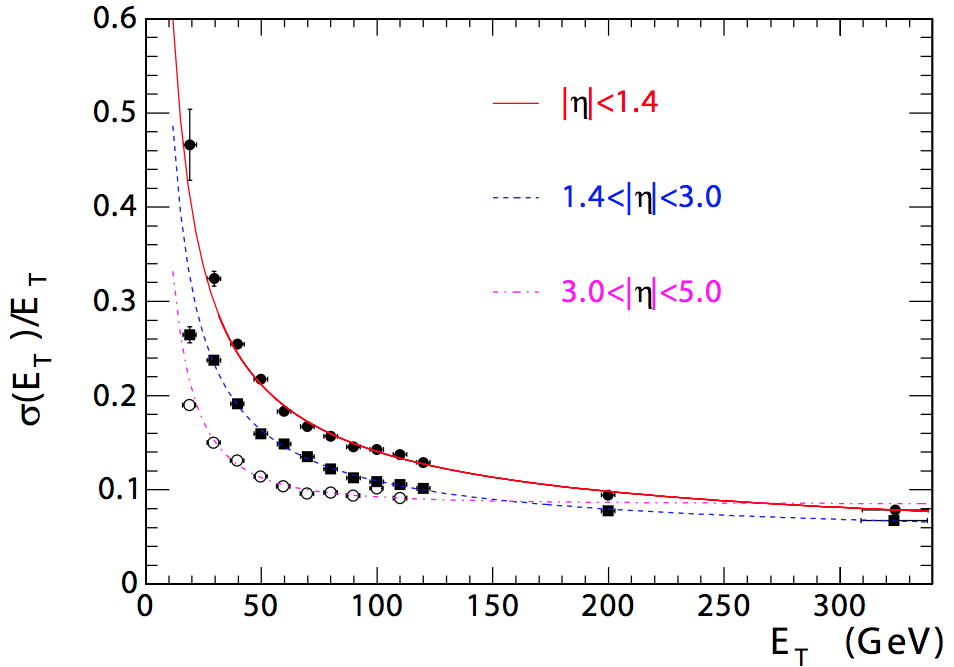
\includegraphics[width=0.7\textwidth]{Figures/CMSHCALRES}
	\caption[The transverse energy resolution of reconstructed jets in the CMS HCAL. It is split into the barrel jets ($\abseta<1.4$), endcap jets ($1.4<\abseta<3.0$) and forward jets ($3.0<\abseta<5.0$)]{The transverse energy resolution of reconstructed jets in the CMS HCAL. It is split into the barrel jets ($\abseta<1.4$), endcap jets ($1.4<\abseta<3.0$) and forward jets ($3.0<\abseta<5.0$) Figure taken from~\cite{CMSExperiment}.}
	\label{fig:CMSHCALRes}
\end{figure}

\subsection{Superconducting magnet}
\label{ssec:Magnet}
% http://iopscience.iop.org/article/10.1088/1748-0221/5/03/T03021/pdf

The solenoid at the heart of CMS is the largest superconducting magnet that has ever been built at 13\m{} long and 6\m{} in diameter.
It is composed from coils of a niobium-titanium alloy wire that are cooled to an operating temperature of 4.5\Kelvin{}. 
It operates at a field strength 3.8\Tesla{} reduced from a design operation field strength of 4\Tesla{} in order to maximise longevity.
The magnet and steel return yokes, which are used to contain the magnetic field, are the most massive components in CMS weighing approximately 12,000 tonnes.
The high field strength allows for very precise measurements of the curvature of charged tracks leading to precise measurements of the momenta of charged particles.

\subsection{Muon detectors}
\label{ssec:MuonChambers}

The muon chambers are the outermost set of detectors at CMS, interleaved with the steel return yoke of the superconducting solenoid.
There are three types of muon chamber present at CMS: resistive plate chambers (RPC), cathode strip chambers (CSC) and drift tubes (DT).
The layout of the muon chambers is presented in Fig.~\ref{fig:CMSMuon}.
\begin{figure}[htpb]
	\centering
	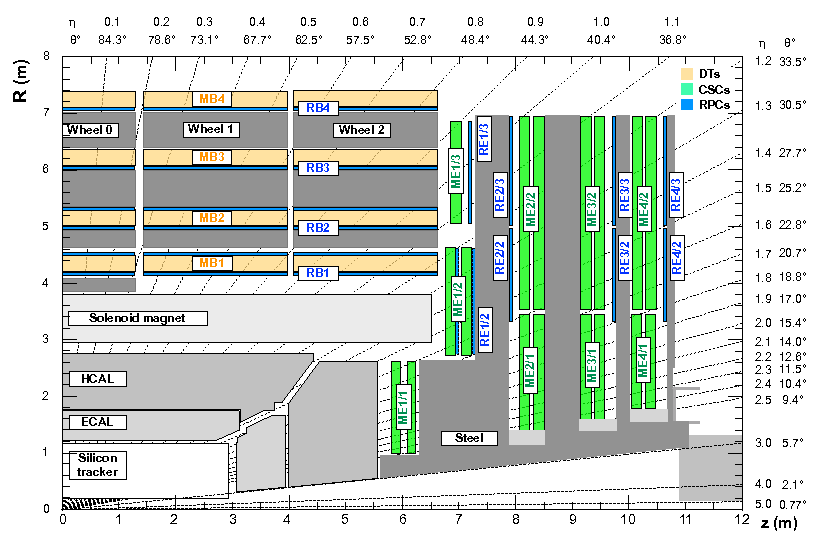
\includegraphics[width=0.95\textwidth]{Figures/CMSMUON}
	\caption[A geometrical one-quarter view of the CMS muon subsystems. The drift tube stations are indicated in yellow the cathode strip chambers in green and the resistive plate chambers in blue.]{A geometrical one-quarter view of the CMS muon subsystems. The drift tube stations are indicated in yellow the cathode strip chambers in green and the resistive plate chambers in blue. Figure taken from~\cite{CMSMuon}.}
	\label{fig:CMSMuon}
\end{figure}

The relatively low muon rates and uniform local magnetic field strengths in the barrel make DT stations a good option for measuring muons in this phase space region covering up to $\abseta<1.2$.
Each cell is $13\times42\mmsq$ containing a gaseous mixture composed of 15\% $\mathrm{CO}_{2}$ and 85\% $\mathrm{Ar}$, with an anode central wire running the length of the cell.
As a charge is left in the cell, liberated electrons drift towards the central wire forming a signal.
The cells arranged into a set of four layers, each offset by half a cell-width to reduce non-sensitive detector regions, in what is know as a superlayer.
A set of three of the superlayers form a DT muon station, where the outer two are aligned parallel to the beam line and the central one perpendicular.
This means the central superlayer can be used to calculate the $z$ co-ordinate and the outer two to measure the co-ordinates in $r,\,\phi$ space.
The DT cells have a high spatial resolution but also a slow drift time of up to 380\ns{}.
% Still very low occ with the high drift time (no mulithits) but large enough to be cost effective
% https://cds.cern.ch/record/1129810/files/jinst8_08_s08004.pdf

In the endcaps where the muon rates are higher, 540 CSCs are employed in the range $0.9<\abseta<2.4$. 
They have trapezoidal shapes to provide contiguous $\phi$ coverage in four disks in each endcap.
The CSCs have a quicker response time, a finer granularity and are less affected by variations in the magnetic field making them preferable to the DTs.
Each CSC station consists of seven layers of cathode panels, each with strips milled running lengthwise at constant $\Delta\phi$ width, interleaved with six layers of azimuthally running anode wires.
The formation of six gas gaps are filled with 40\% $\mathrm{Ar}$, 50\% $\mathrm{CO}_{2}$ and 10\% $\mathrm{CF}_{4}$.
As a charged muon passes through the gas, electrons travel to the anode wires and ions to the cathode strips providing the co-ordinates in $r,\,\phi$ space.

Finally, 610 RPCs are found in both the barrel (six layers) and endcaps (four layers) up to $\abseta<1.8$.
They are composed of gaseous parallel-plate detectors with two gas gaps filled with a mixture of 96.2\% $\mathrm{C}_{2}\mathrm{H}_{2}\mathrm{F}_{4}$, 3.5\% iso-$\mathrm{C}_{4}\mathrm{H}_{10}$ and 0.3\% $\mathrm{SF}_{4}$, separated by a common charge read-out strips.
The RPCs have adequate spatial resolution, however they are complimentary to the DTs and CSCs due to their very fast response time ($\approx2\ns$) which is much faster than the time it takes for the bunch crossing.
This makes the RPCs ideal detectors for triggering muons, able to unambiguously identify the relevant bunch crossing a muon track is associated to.
Each component is discussed in more detail in~\cite{CMSExperiment,CMSMuon}.
% Double gap means each single gap operates at lower high voltage (gain) and higher detector efficiency.

Figure~\ref{fig:CMSMuonRes} shows the expected momentum resolution of the muons based on tracker information only, muon chamber information only and a combination of tracker and muon chamber information.
At low muon \pt{} the resolution is driven from the reconstruction of muons in the tracker, however as the \pt{} of the muon increases then the combination of information from the tracker and muon chambers results in improved resolution.

\begin{figure}[htpb]
	\centering
	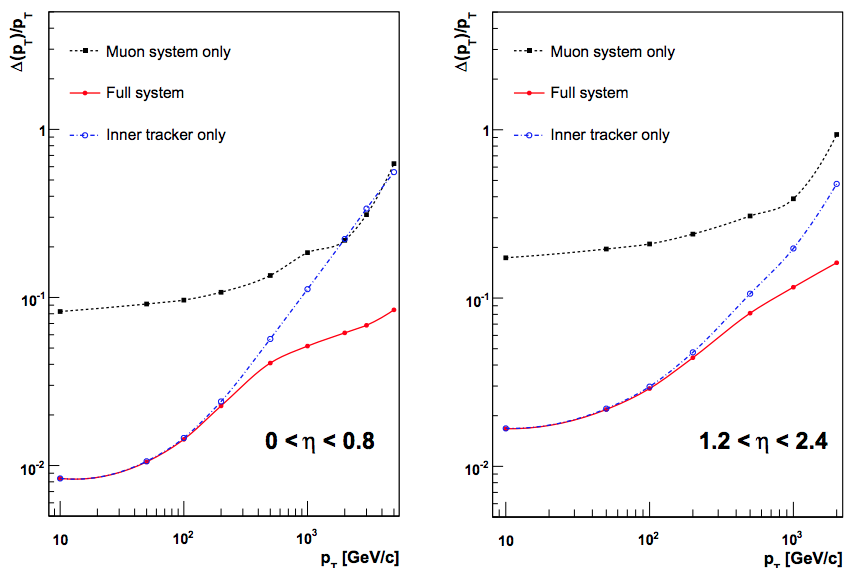
\includegraphics[width=0.85\textwidth]{Figures/CMSMUONRES}
	\caption[The muon \pt{} resolution as a function of \pt{} using the tracking only, muon subdetectors only or both.]{The muon \pt{} resolution as a function of \pt{} using the tracking only, muon subdetectors only or both. Figure taken from~\cite{CMSExperiment}.}
	\label{fig:CMSMuonRes}
\end{figure}
% Is this figure expected or data? I think expected...
% TODO GEMS?

\subsection{Triggers}
\label{ssec:Trig}

The CMS detector produces events at an approximate rate of 40\MHz{}. 
If each reconstructed event has a size of $\sim1\unit{MB}$, then data would be produced at a rate of 40~$\mathrm{TB}~\mathrm{s}^{-1}$. 
It is not feasible to fully reconstruct and store the full rate of data production so a method of data reduction, called triggering, is used. 
Triggering decides on an event-by-event basis whether a collision is likely to be highly-energetic and interesting, or just an elastic collision or low-energy QCD process. 
There are two types of triggering systems at CMS, the Level-1 hardware triggers (L1T) and the High-Level software triggers (HLT). 

The L1T must decide within 3.2\us{} of an event occurring whether it should be rejected of tentatively accepted.
The schematic workflow of the L1T is shown in Fig.~\ref{fig:CMSL1T}.
It uses only basic information from the detector known as \textit{trigger primitives} to make a decision.
These trigger primitives are formed from the calorimeter deposits and the hits in the muon detectors.
There are two trigger subsystems to the L1T, the calorimeter trigger and the muon trigger.
These access the trigger primitives from different subdetectors and operate independently, with the exception of information passed from the calorimeter trigger to the muon trigger for the computation of muon isolation.
The outcome of both trigger components is then passed to the L1 \textit{global trigger} which makes the final decision on the event.
The L1T reduces the event rate from 40\MHz{} to 100\unit{kHz}, which provides enough latency for the events to be fully reconstructed before being processed by the HLT. 
\begin{figure}[htpb]
	\centering
	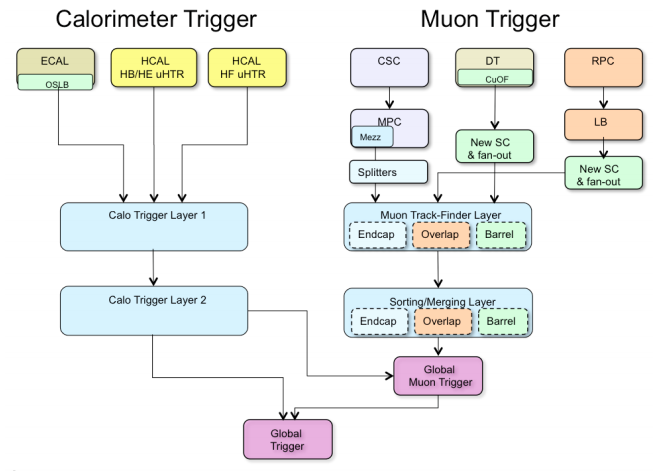
\includegraphics[width=0.85\textwidth]{Figures/CMSL1TUpgrade}
	\caption[A schematic representing the process flow of the L1T. On the left is the calorimeter trigger and on the right the muon trigger which operate on independent trigger primitives. The final decision is taken by the global trigger using all information available.]{A schematic representing the process flow of the L1T. On the left is the calorimeter trigger and on the right the muon trigger which operate on independent trigger primitives. The final decision is taken by the global trigger using all information available \cite{CMS:L1TUpgradeTDR}.}
	\label{fig:CMSL1T}
\end{figure}

The L1T runs approximately 200 trigger algorithms, the outcomes of which form the \textit{seeds} for the HLT. 
The HLT with access to the L1 seeds, full collision kinematics and composition, reduces the final physics production rate to 1\unit{kHz} and classifies the events with respect to specific topologies.
The events are collected into data sets containing similar topologies, for example sets with a single isolated electron or sets that have high jet multiplicities.

\subsection{Computational power} % (fold)
\label{sub:computational_power}

The amount of raw data produced by the LHC and the number of large simulations generated for analyses is far too much for a single storage site to be viable.
Therefore the Worldwide LHC Computing Grid (WLCG) was produced to share the burden.
The WLCG is a tiered system with all raw data being stored at a central Tier-0 computing facility and subsequently distributed to Tier-1 and Tier-2 sites in the countries and institutes affiliated to CERN.

The complete set of raw data is stored at the CERN Tier-0 data centre, where the combined permanent archive stored on tape breached 200\unit{Pb} on the 29th June 2017.
In terms of online storage the data centre at CERN holds 45\unit{Pb} with a further 5.5\unit{Pb} extension at the Wigner Research Centre for Physics in Budapest.
The 100,000 processor cores at the data centre deal with 1\unit{Pb} of data every day.

The large Tier-1 facilities store a large fraction of the data and simulation sets so that there are multiple redundancies for every data set.
The 13 Tier-1 facilities are the main workhorses of the WLCG performing large-scale reprocessing of the raw data sets and the generation of simulated events.

Tier-2 sites, of which there are 155, store data sets distributed to them from Tier-1 facilities and specific data sets that are useful for locally based analysis teams.
They provide a moderate number of processor cores for computational tasks, most generally for the production of simulated events.
The distributed nature of the file system allows for any person to access data sets from any site which has it stored and to use free computational power anywhere that is part of the WLCG, increasing the overall computational efficiency.

% subsection computational_power (end)

\subsection{Data collection in 2016} % (fold)
\label{sub:data_collection_in_2016}

As already stated in Sec.~\ref{sec:lumi}, an integrated luminosity of \Lumi{} was collected by CMS in 2016.
To further classify the data used in this thesis, Tab.~\ref{tb:Data2016} shows the data collected with respect to the run period.
A run period refers to periods of similar data taking throughout the year.
Run period A is used for the commissioning of the detector.
Run periods often change after a short technical stop has occurred.
\begin{table}
	\centering
	\caption{The sets of single electron and single muon data collected during 2016 split into individual runs. A total luminosity of 35.9\fbinv{} of data was collected.}
	\label{tb:Data2016}
	\resizebox{\linewidth}{!}{%
	\begin{tabular}{llcc}
		\textbf{Channel}		&	\textbf{Data set}				& \textbf{Run ranges}	& \textbf{Luminosity (\fbinv{})} \\
		\hline
		SingleElectron(Muon)	 &	Run2016B-03Feb2017\_ver2-v2		& 272007--275376		&	5.79 \\
								 &	Run2016C-03Feb2017-v1			& 275657--276283		&	2.57 \\
								 &	Run2016D-03Feb2017-v1			& 276315--276811		&	4.25 \\
								 &	Run2016E-03Feb2017-v1			& 276831--277420		&	4.01 \\
								 &	Run2016F-03Feb2017-v1			& 277772--278808		&	3.10 \\
								 &	Run2016G-03Feb2017-v1			& 278820--280385		&	7.54 \\
								 &	Run2016G-03Feb2017-ver2(3)-v1	& 280919--284044		&	8.61 \\
		\hline
		Total integrated luminosity	 &	&  & 35.87 \\
	\end{tabular}%
	}
\end{table}

The initial data sets used in this thesis are classified as containing either a single electron or a single muon.
On these data sets a preselection is made via the HLT selection.
In the \eJets{} channel the trigger requires there to be an electron with a $\pt>32\GeV$, a $\abseta<2.1$ and to pass a set of tight identification requirements (\eTrigger{}).
In the \muJets{} channel an isolated global muon or isolated tracker muon is required with a $\pt > 24\GeV$ and a $\abseta < 2.4$ (\muTrigger{}).




% subsection data_collection_in_2016 (end)

% Figure~\ref{CMSL1T} shows the 

% \begin{figure}[htpb]
% 	\centering
% 	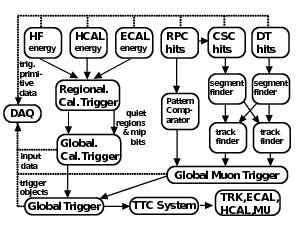
\includegraphics[width=0.7\textwidth]{Figures/CMSL1T}
% 	\caption[This needs a caption TODO Add ref in text]{This needs a caption TODO Add ref in text~\cite{CMSL1T}.}
% 	\label{fig:CMSL1T}
% \end{figure}

% \subsection{UpgradesToCome}
% \label{ssec:Upgrade}
% Track Trigger?
% \subsection{DataTaken}
% \label{ssec:DataTaken}
